% ============================================================
%  Estadística · LCC · Universidad de Sonora
%  Semana 1 — Presentación del curso, el conjunto penguins, R y RStudio
%  Archivo autocontenido. Se puede copiar y pegar tal cual en Overleaf.
% ============================================================
\documentclass[aspectratio=169,10pt]{beamer}
\usepackage[utf8]{inputenc}
\usepackage[T1]{fontenc}
\usepackage[spanish,es-nodecimaldot,es-noquoting]{babel}
\usepackage{lmodern}
\usepackage{amsmath,amssymb}
\usepackage{booktabs}
\usepackage{tikz}
\usepackage{listings}
\usepackage{graphicx}
\graphicspath{{figuras/}}
% ------------------------------------------------------------
%  ILUSTRACIONES DE palmerpenguins
%  Ejecutar una vez  presentaciones/copiar-figuras.R  para obtenerlas.
%  Si no están presentes, las diapositivas compilan igual usando los
%  dibujos en TikZ definidos más abajo.
%  Crédito obligatorio: Artwork by @allison_horst
% ------------------------------------------------------------
\newcommand{\creditoHorst}{{\tiny\color{grisT} Ilustración: \textit{Artwork by @allison\_horst}}}
% ---------- Tema y colores ----------
\usetheme{default}
\setbeamertemplate{navigation symbols}{}
\definecolor{azulUS}{HTML}{1F4E79}
\definecolor{azulClaro}{HTML}{DCE6F1}
\definecolor{grisT}{HTML}{5F5E5A}
\definecolor{negroP}{HTML}{2B2B2B}
\definecolor{picoNaranja}{HTML}{E8871E}
\definecolor{rosaK}{HTML}{F4A6B8}
\definecolor{verdeOk}{HTML}{1D9E75}
\definecolor{rojoAc}{HTML}{C0392B}
\definecolor{grisR}{HTML}{9A9A9A}
\definecolor{azulR}{HTML}{2266B3}
\setbeamercolor{structure}{fg=azulUS}
\setbeamercolor{frametitle}{fg=white,bg=azulUS}
\setbeamercolor{title}{fg=azulUS}
\setbeamerfont{frametitle}{size=\large,series=\bfseries}
\setbeamertemplate{frametitle}{%
  \nointerlineskip
  \begin{beamercolorbox}[wd=\paperwidth,ht=2.6ex,dp=1.2ex,leftskip=0.3cm]{frametitle}
    \usebeamerfont{frametitle}\insertframetitle
  \end{beamercolorbox}}
\setbeamertemplate{footline}{%
  \hfill\textcolor{grisT}{\tiny Estadística · LCC · Unison \quad
  \insertframenumber/\inserttotalframenumber}\hspace{0.3cm}\vspace{0.15cm}}
\setbeamertemplate{itemize item}{\textcolor{azulUS}{\raisebox{0.15ex}{\tiny$\blacksquare$}}}
\setbeamertemplate{itemize subitem}{\textcolor{grisT}{\raisebox{0.15ex}{\tiny$\bullet$}}}
% ---------- Estilo para código de R ----------
\lstdefinestyle{Rstyle}{
  language=R, basicstyle=\ttfamily\footnotesize,
  keywordstyle=\color{azulUS}\bfseries, commentstyle=\color{grisT}\itshape,
  stringstyle=\color{verdeOk}, showstringspaces=false, breaklines=true,
  frame=single, rulecolor=\color{azulClaro}, backgroundcolor=\color{azulClaro!35},
  numbers=none, aboveskip=6pt, belowskip=4pt,
  % Para que las vocales acentuadas no rompan la compilación si algún día se
  % escriben dentro de un bloque de código o de un comentario.
  extendedchars=true,
  literate={á}{{\'a}}1 {é}{{\'e}}1 {í}{{\'i}}1 {ó}{{\'o}}1 {ú}{{\'u}}1
           {Á}{{\'A}}1 {É}{{\'E}}1 {Í}{{\'I}}1 {Ó}{{\'O}}1 {Ú}{{\'U}}1
           {ñ}{{\~n}}1 {Ñ}{{\~N}}1 {ü}{{\"u}}1 {Ü}{{\"U}}1
           {¿}{{?`}}1 {¡}{{!`}}1}
\lstset{style=Rstyle}
% ---------- Comandos de R dentro del texto ----------
%  Mismo aspecto que el código en línea del libro: fondo gris y letra morada.
%  Los valores vienen del tema del libro (--bs-code-color: #7D12BA). El gris se
%  oscureció un poco respecto al de la web (#F8F9FA) para que se vea proyectado.
\definecolor{codigoTexto}{HTML}{7D12BA}
\definecolor{codigoFondo}{HTML}{EFF0F2}
\newcommand{\Rc}[1]{{\setlength{\fboxsep}{1.6pt}%
  \colorbox{codigoFondo}{\textcolor{codigoTexto}{\texttt{#1}}}}}
% ---------- Interruptor de las diapositivas de respuestas ----------
%  Con \respuestastrue el PDF sale completo, como para dar la clase.
%  Con \respuestasfalse desaparecen las dos diapositivas de respuestas de la
%  práctica, que es la versión que conviene compartir mientras la tarea sigue
%  abierta. Basta cambiar esa palabra y volver a compilar.
\newif\ifrespuestas
\respuestastrue
% ---------- Caja auxiliar para destacar ideas ----------
\newcommand{\destaca}[1]{%
  \par\vspace{3pt}\noindent
  \colorbox{azulClaro}{%
    \parbox{\dimexpr\linewidth-2\fboxsep\relax}{\vspace{3pt}#1\vspace{3pt}}}%
  \par\vspace{3pt}}
% ---------- Hojas de separación por sesión ----------
%  Cumplen dos funciones: al preparar la clase, ver de un golpe dónde terminó
%  cada día; al repasar, reconocer dónde empieza cada bloque.
%
%  SIN NUMERAR A PROPÓSITO. El número global de sesión se rompe en cuanto el
%  calendario real se mueve, y se mueve siempre. La hoja marca el corte por su
%  posición, que no depende de ninguna cuenta.
%
%  Uso:  \hojaSesion{Título del bloque}{Resumen de lo que se vio.}
%  Va dentro de un frame [plain]:
%      \begin{frame}[plain]
%        \hojaSesion{...}{...}
%      \end{frame}
\newcommand{\hojaSesion}[2]{%
  \vfill
  \begin{beamercolorbox}[wd=\textwidth,sep=16pt,center]{frametitle}
    {\Large\bfseries #1}\\[11pt]
    \begin{minipage}{0.82\textwidth}\centering\small #2\end{minipage}
  \end{beamercolorbox}
  \vfill}
% ============================================================
%  PINGÜINOS EN TIKZ  (estilo kawaii)
%  Solo se usan como respaldo: si están las ilustraciones de Horst en
%  figuras/, esas tienen prioridad y estos dibujos no aparecen.
% ============================================================
% Cuerpo común. Argumento: color de pico y patas.
\newcommand{\cuerpoPing}[1]{%
  \fill[negroP] (-0.88,0.18) ellipse (0.17 and 0.5);      % ala izquierda
  \fill[negroP] (0.88,0.18) ellipse (0.17 and 0.5);       % ala derecha
  \fill[#1] (-0.28,-1.12) ellipse (0.19 and 0.085);       % pata izquierda
  \fill[#1] (0.28,-1.12) ellipse (0.19 and 0.085);        % pata derecha
  \fill[negroP] (0,0) ellipse (0.82 and 1.1);             % cuerpo
  \fill[white] (0,-0.16) ellipse (0.53 and 0.82);         % vientre
}
% Ojos grandes con brillo y rubor
\newcommand{\ojosPing}{%
  \fill[white] (-0.22,1.3) circle (0.155);
  \fill[white] (0.22,1.3) circle (0.155);
  \fill[negroP] (-0.20,1.28) circle (0.085);
  \fill[negroP] (0.24,1.28) circle (0.085);
  \fill[white] (-0.235,1.315) circle (0.032);
  \fill[white] (0.205,1.315) circle (0.032);
  \fill[rosaK,opacity=0.55] (-0.44,1.10) circle (0.085);
  \fill[rosaK,opacity=0.55] (0.44,1.10) circle (0.085);
}
\newcommand{\picoPing}[1]{%
  \fill[#1] (-0.10,1.13) -- (0.10,1.13) -- (0,0.94) -- cycle;
}
% --- Adelaida (Adelie): cabeza negra, anillo blanco alrededor del ojo
\newcommand{\pingAdelie}{%
  \begin{scope}
    \cuerpoPing{picoNaranja}
    \fill[negroP] (0,1.22) circle (0.6);
    \fill[white] (-0.22,1.3) circle (0.20);
    \fill[white] (0.22,1.3) circle (0.20);
    \ojosPing
    \picoPing{picoNaranja}
  \end{scope}}
% --- Barbijo (Chinstrap): cara blanca con una franja negra bajo el mentón
\newcommand{\pingChinstrap}{%
  \begin{scope}
    \cuerpoPing{picoNaranja}
    \fill[negroP] (0,1.22) circle (0.6);
    \fill[white] (0,1.26) ellipse (0.5 and 0.5);
    \draw[negroP,line width=1.6pt] (-0.44,1.02) arc (205:335:0.48);
    \ojosPing
    \picoPing{negroP}
  \end{scope}}
% --- Juanito (Gentoo): parche blanco sobre los ojos y pico naranja
\newcommand{\pingGentoo}{%
  \begin{scope}
    \cuerpoPing{picoNaranja}
    \fill[negroP] (0,1.22) circle (0.6);
    \fill[white] (-0.26,1.5) ellipse (0.21 and 0.13);
    \fill[white] (0.26,1.5) ellipse (0.21 and 0.13);
    \fill[white] (0,1.56) ellipse (0.3 and 0.075);
    \ojosPing
    \picoPing{picoNaranja}
  \end{scope}}
% ============================================================
%  ICONOS DE R Y RSTUDIO
%  Aproximaciones estilizadas hechas en TikZ. Si se prefieren los
%  logotipos oficiales, están disponibles en r-project.org (CC-BY-SA)
%  y en posit.co; bastaría guardarlos en figuras/ e incluirlos.
% ============================================================
\newcommand{\iconoR}{%
  \begin{scope}
    \fill[grisR] (0,0) ellipse (0.72 and 0.50);
    \fill[white] (0,0) ellipse (0.50 and 0.31);
    \node[azulR,font=\bfseries\large] at (0.02,0.02) {R};
  \end{scope}}
\newcommand{\iconoRStudio}{%
  \begin{scope}
    \fill[azulR] (0,0) circle (0.52);
    \fill[white] (0,0) circle (0.40);
    \node[azulR,font=\bfseries] at (0,0.02) {R};
    \draw[azulR,line width=1.3pt] (-0.20,-0.26) -- (0.28,-0.26);
  \end{scope}}
% ============================================================
\title{\LARGE\textbf{Estadística}}
\subtitle{Licenciatura en Ciencias de la Computación}
\author{Prof. Rosalía Gpe. Hernández Amador}
\institute{Departamento de Matemáticas · Universidad de Sonora}
\date{Semestre 2026-2}
\begin{document}
% ============================================================
\begin{frame}[plain]
  \titlepage
\end{frame}
% ============================================================
\section{Presentación del curso}
% ---------- bloque: presentación del curso ----------
\begin{frame}[plain]
  \hojaSesion{Presentación del curso}{%
  Qué estudia la Estadística y cómo está organizado el curso. El libro de texto, el mapa de decisión y el formulario. Con qué conjuntos de datos vamos a trabajar, el
  proyecto de la cata a ciegas, los criterios de evaluación, y por qué el
  software del curso es R.}
\end{frame}
\begin{frame}{Medios de contacto}
\begin{itemize}
    \item \textbf{Prof. Rosalía Gpe. Hernández Amador}\\
      {\small Correo institucional: rosalia.hernandez@unison.mx}\\
      {\small Ubicación: Edificio 3K2, Módulo 9, Cubículo 1}
      \vspace{0.25cm}
    \item \textbf{Teams}: avisos, recordatorios y material del curso
      \vspace{0.25cm}
    \item \textbf{Ramanujan} (Moodle): cuestionarios y entregas
      \vspace{0.25cm}
    \item \textbf{Libro del curso} (en construcción):\\
      {\small \url{https://rosaliahdez.github.io/notas-estadistica/}}
\end{itemize}
      \vspace{0.2cm}
\end{frame}
% ============================================================
\begin{frame}{¿De qué trata la Estadística?}
  La Estadística es el área de las matemáticas que estudia las técnicas que nos permiten \textbf{obtener conocimiento a partir de datos}. Para lograr ésto, se requieren de tres acciones clave:
  \vspace{0.5cm}
  \begin{columns}[T]
    \begin{column}{0.32\textwidth}
      \destaca{\centering\textbf{Analizar}\\[3pt]
      {\small Organizar, resumir y visualizar lo que ya tenemos}}
    \end{column}
    \begin{column}{0.32\textwidth}
      \destaca{\centering\textbf{Producir datos}\\[3pt]
      {\small De dónde vienen los datos importa tanto como lo que hacemos con ellos}}
    \end{column}
    \begin{column}{0.32\textwidth}
      \destaca{\centering\textbf{Inferir}\\[3pt]
      {\small Decir algo sobre el todo habiendo visto solo una parte}}
    \end{column}
  \end{columns}
\vspace{5mm}
La Probabilidad es el \textbf{fundamento teórico} en el que se basan las técnicas estadísticas. Por esta razón, el curso de probabilidad antecede a éste.
\end{frame}
% ============================================================
\begin{frame}{Estructura del temario del curso}
  El temario oficial del curso se divide en tres partes principales:

  \vspace{4mm}

  \begin{center}
  \begin{tikzpicture}[scale=1]
    \node[fill=azulClaro,rounded corners,text width=3.4cm,align=center,minimum height=2.1cm] (a) at (-4.2,0)
      {\textbf{I. Exploración}\\[3pt]{\scriptsize Unidades 1--3}\\[3pt]{\scriptsize Mirar y resumir datos}};
    \node[fill=azulClaro,rounded corners,text width=3.4cm,align=center,minimum height=2.1cm] (b) at (0,0)
      {\textbf{II. Producción}\\[3pt]{\scriptsize Unidades 4--5}\\[3pt]{\scriptsize Muestreo y experimentos}};
    \node[fill=azulClaro,rounded corners,text width=3.4cm,align=center,minimum height=2.1cm] (c) at (4.2,0)
      {\textbf{III. Inferencia}\\[3pt]{\scriptsize Unidades 6--11}\\[3pt]{\scriptsize De la muestra a la población}};
    \draw[->,azulUS,very thick] (a) -- (b);
    \draw[->,azulUS,very thick] (b) -- (c);
  \end{tikzpicture}
  \end{center}

  \vspace{0.4cm}

  Cada parte corresponde a un área distinta de la Estadística. La parte I es
  \textit{Estadística Descriptiva}, la parte II introduce el \textit{Muestreo} y el
  \textit{Diseño de Experimentos}, y la parte III es \textit{Estadística Inferencial}.

  \vspace{0.8cm}
  {\footnotesize El temario completo del curso puede consultarse en la página del
  programa de la licenciatura:\\
  \href{https://cc.unison.mx/plan-de-estudios/}{\texttt{lcc.unison.mx/plan-de-estudios}}.}

\end{frame}
% ============================================================
\begin{frame}{Objetivos del curso}
  \begin{columns}[T]
    \begin{column}{0.48\textwidth}
      \textcolor{rojoAc}{\textbf{NO se busca}}
      \begin{itemize}
        \item Que memoricen fórmulas
        \item Que apliquen procedimientos sin saber por qué
        \item Que reporten un valor y se sientan satisfechos
      \end{itemize}
    \end{column}
    \begin{column}{0.48\textwidth}
      \textcolor{verdeOk}{\textbf{Lo que SÍ se busca}}
      \begin{itemize}
        \item Que sepan \textbf{qué técnica} corresponde a cada pregunta
        \item Que \textbf{verifiquen los supuestos} antes de confiar en un resultado
        \item Que sepan \textbf{interpretar} y explicárselo a alguien que no es estadístico
      \end{itemize}
    \end{column}
  \end{columns}
\end{frame}
% ============================================================
\begin{frame}{Libro de texto}
  Existe mucha literatura de Estadística, y toda buena fuente sirve para consultar. Sin embargo, este curso se basa en:
  \destaca{Las \textbf{Notas de Estadística} de la Dra.~Gudelia Figueroa Preciado y el
  M.C.~Marco Antonio Valencia Arvizu, material referente de esta asignatura en nuestro  Departamento de Matemáticas.}
  Esas notas fueron la base para crear el \textbf{libro digital} de acceso abierto que usaremos en el curso:
\begin{center}
\href{https://rosaliahdez.github.io/notas-estadistica/}{\texttt{rosaliahdez.github.io/notas-estadistica}}
\end{center}
que conserva la organización de las notas mencionadas, a las cuales se les ha agregado:
  \begin{itemize}
    \item Todo el cómputo en \textbf{R}, con el código explícito
    \item \textbf{Gráficos interactivos} para mover parámetros y analizar su efecto
    \item Ejercicios \textbf{con soluciones explicadas}
    \item Un \textbf{mapa de decisión} para orientar sobre la técnica adecuada en cada escenario
    \item Un \textbf{formulario} con todas las fórmulas del curso
  \end{itemize}
\end{frame}
% ============================================================
\begin{frame}{Sobre el mapa de decisión}
  Cada tema aporta un renglón a esta tabla, que nombramos \textbf{mapa de decisión} y que iremos armando a lo largo del curso:
  
  \vspace{0.35cm}
  \centering
  {\small
  \begin{tabular}{@{}p{5.1cm}p{3.6cm}p{4.1cm}@{}}
    \toprule
    \textbf{Mi pregunta} & \textbf{Tipo de datos} & \textbf{Técnica} \\
    \midrule
    ¿Cómo se distribuye esta variable? & 1 cuantitativa & Histograma, caja, Q-Q plot \\
    ¿Difieren dos grupos? & Cuantitativa por 2 grupos & Prueba $t$ \\
    ¿Difieren tres o más grupos? & Cuantitativa por $k$ grupos & ANOVA y post-hoc \\
    ¿Están asociadas dos categóricas? & Tabla de contingencia & Ji-cuadrada \\
    \multicolumn{3}{c}{\textcolor{grisT}{\textit{... y doce renglones más}}} \\
    \bottomrule
  \end{tabular}}
  \vspace{0.5cm}
  \raggedright
  \destaca{La pregunta importante en el curso no será \textit{``¿cuál es la fórmula?''},
  sino \textbf{\textit{``¿qué técnica corresponde a esta pregunta y a estos datos?''}}

  \vspace{0.15cm}
  Nótese la columna de en medio. El mapa no se consulta con las palabras del problema
  sino con el \textbf{tipo de las variables}, y eso se irá haciendo evidente conforme lo
  vayamos armando.}
\end{frame}
\begin{frame}{Sobre el formulario}
  También, conforme avancemos en el curso, se irá construyendo un formulario (que se utilizará durante los exámenes). Se presenta aquí un pequeño extracto:
  \vspace{0.3cm}
    \begin{columns}[T]
    \begin{column}{0.48\textwidth}
      {\footnotesize \textbf{Media y varianza muestrales}}
      \vspace{-0.15cm}
      \begin{align*}
        \bar{x} &= \frac{\sum_{i=1}^{n} x_i}{n} \\[4pt]
        s^2 &= \frac{1}{n-1}\left[\sum_{i=1}^{n} x_i^2 - n\bar{x}^2\right]
      \end{align*}
      {\color{grisT}\small En R:}~\Rc{mean(x)}~~\Rc{var(x)}
    \end{column}
    \begin{column}{0.48\textwidth}
      \raggedright
      {\footnotesize \textbf{Prueba para una media}}
      \vspace{-0.15cm}
      \begin{align*}
        t_c &= \frac{\bar{x} - \mu_0}{s/\sqrt{n}}, \qquad \text{gl} = n-1
      \end{align*}
      {\color{grisT}\small En R:}~\Rc{t.test(x, mu = mu0)}
    \end{column}
  \end{columns}
  \vspace{0.4cm}
      \destaca{ Cada fórmula aparece acompañada de su correspondiente comando en R. El formulario completo se encuentra en los apéndices del libro y se puede imprimir.}
\end{frame}
% ============================================================
\begin{frame}{Con qué datos vamos a trabajar}
  Para no cambiar de contexto en cada ejemplo (como se suele hacer en libros aplicados de Estadística) usaremos \textbf{pocos conjuntos de datos muchas veces}.
  \vspace{0.4cm}

  \centering
  {\small
  \begin{tabular}{@{}p{3.5cm}p{8.5cm}@{}}
    \toprule
    \textbf{Conjunto} & \textbf{Qué es} \\
    \midrule
    \textbf{Pingüinos} & %344 pingüinos de la Antártida.
    Datos reales y limpios. El dataset base para nuestras prácticas \\
    \textbf{Galletas} & Cata a ciegas diseñada y ejecutada por los estudiantes del curso \\
    \textbf{Lagartijas} & Fisiología de ejemplares de ciudad contra campo abierto \\
    \textbf{Rickettsiosis} & Zona de residencia, contacto con perros y garrapatas frente al resultado de laboratorio \\
    \textbf{Algoritmos} & Tiempos de ejecución de un algoritmo, según el tamaño de la entrada y según el equipo \\
    \bottomrule
  \end{tabular}}
  \vspace{0.5cm}
  \raggedright

 \destaca{Se trabajarán a lo largo del curso, aplicando las técnicas correspondientes al tipo de datos y a las preguntas que se buscan resolver.
 
\vspace{2mm}
  Primero describiremos los datos, luego entenderemos cómo se produjeron (expositores invitados), y al final se harán inferencias.}
\end{frame}
% ============================================================
\begin{frame}{El proyecto final del curso: una cata a ciegas}
  \begin{columns}[T]
    \begin{column}{0.55\textwidth}
      Vamos a diseñar y ejecutar un \textbf{experimento real}: evaluar si cuatro
      marcas de galletas gustan por igual.
      \vspace{0.3cm}
      \begin{itemize}
        \item Ustedes diseñan el experimento
        \item Lo ejecutamos en grupo
        \item Lo analizamos con ANOVA
        \item Lo reportan y lo presentan
      \end{itemize}
    \end{column}
    \begin{column}{0.42\textwidth}
      \destaca{\small Preguntas que tendrán que resolver ustedes:
      \vspace{0.2cm}

      ¿En qué orden prueba cada juez? ¿Deben saber qué marca están probando? ¿Cuántas personas hacen falta?}
    \end{column}
  \end{columns}
  \vspace{0.4cm}
   \destaca{Al final del curso tendrán un estudio propio, de principio a fin, ejemplificando así el \textbf{ciclo completo de un estudio estadístico}.}
\end{frame}
% ============================================================
\begin{frame}{Criterios de evaluación del curso}

  \centering
  {\small
  \begin{tabular}{@{}p{5.4cm}c p{5.9cm}@{}}
    \toprule
    \textbf{Instrumento} & \textbf{Valor} & \textbf{Notas} \\
    \midrule
    Exámenes parciales (3-4) & 45\,\% & En papel, con formulario \\
    Proyecto de la cata & 25\,\% & Diseño, ejecución, reporte y presentación \\
    Cuestionarios por unidad & 20\,\% & En Moodle, con varios intentos \\
    Prácticas en R & 10\,\% & Actividades cortas en clase y/o casa \\
    \midrule
    \textbf{Total} & \textbf{100\,\%} & \\
    \bottomrule
  \end{tabular}}
  \vspace{0.5cm}
  \raggedright
  \destaca{Los exámenes se aplican con formulario. No se evalúa memorización, sino que sepan \textbf{elegir la técnica}, verificar supuestos, \textbf{calcular} sobre conjuntos pequeños de datos, \textbf{interpretar salidas de R}, y \textbf{explicar} la conclusión en lenguaje simple, entendible por alguien que no es estadístico.}
\vspace{0.3cm}
  {\footnotesize Para tener derecho a evaluación ordinaria se requiere al menos el \textbf{75 \% de asistencia}, conforme al Artículo 70 del Reglamento Escolar de la Universidad de Sonora.}
\end{frame}
% ============================================================
\begin{frame}{Software principal: R · Interfaz: RStudio}
  \begin{columns}[T]
    \begin{column}{0.5\textwidth}
      \textbf{¿Por qué R y no Python?}
      \begin{itemize}
        \item Se usa en biología, salud, economía y ciencias sociales:
          áreas donde probablemente les toque colaborar
        \item Se pueden crear libretas reproducibles en lenguaje Markdown
        \item Se integra con Quarto para escribir reportes vistosos, dashboards, presentaciones \dots
      \end{itemize}
      \vspace{0.2cm}
    \end{column}
    \begin{column}{0.47\textwidth}
      \textbf{¿Y RStudio?}
      \begin{itemize}
        \item Es el \textbf{entorno de trabajo} donde se usa R. La interfaz de RStudio tiene a la mano consola, editor,
        gráficas y gestor de archivos en una sola ventana
        \item R es el motor de RStudio.
      \end{itemize}
      \raggedright
    \end{column}
  \end{columns}
      \destaca{ El objetivo no es aprender a programar en R, sino aprender a utilizar los comandos estadísticos básicos de R para analizar datos y hacer inferencia.}
  \vspace{0.3cm}
  {\footnotesize Para quien venga de Python: en los apéndices del libro hay una tabla de
  equivalencias entre los comandos centrales de R y sus contrapartes en Python.}
\end{frame}
\begin{frame}{Formas de usar R}
  \begin{center}
  {\small
  \begin{tabular}{@{}p{3.1cm}p{4.7cm}p{4.4cm}@{}}
    \toprule
    \textbf{Opción} & \textbf{Cuándo conviene} & \textbf{Qué requiere} \\
    \midrule
    \textbf{El libro del curso} & Para corridas rápidas, incluso desde el celular &
      No ocupa instalación, se ejecuta en el navegador \\
    \textbf{R en la terminal} & Si nos sentimos cómodos trabajando desde la terminal &
      Instalar R \\
    \textbf{R + RStudio} & Cuando queremos escribir código, ver gráficas y administrar archivos en una sola ventana &
    Instalar R y luego RStudio \\
          \textbf{Posit Cloud} & Trabajar sin instalar, desde cualquier máquina &
      Crear una cuenta gratuita \\
    \bottomrule
  \end{tabular}}
  \end{center}

  \vspace{5mm}
  \destaca{
   \textbf{Tarea: Instalar R y luego RStudio}, en ese orden:
  \begin{itemize}
    \item R: \texttt{https://cran.r-project.org}
    \item RStudio Desktop: \texttt{https://posit.co/download/rstudio-desktop}
    \end{itemize}}
\end{frame}

% ============================================================
\section{El conjunto de datos penguins}
% ---------- bloque: el conjunto penguins ----------
\begin{frame}[plain]
  \hojaSesion{De dónde salen los datos: \texttt{penguins}}{%
  El dataset que usaremos a lo largo del curso. La estación Palmer y las tres
  especies, qué se midió y con qué instrumento, el diccionario de variables, el
  diseño del estudio, por qué hay datos faltantes y por qué entender el contexto
  es parte del análisis.}
\end{frame}
\begin{frame}{Los pingüinos de Palmer}
  \begin{center}
  \IfFileExists{figuras/lter_penguins.png}{%
    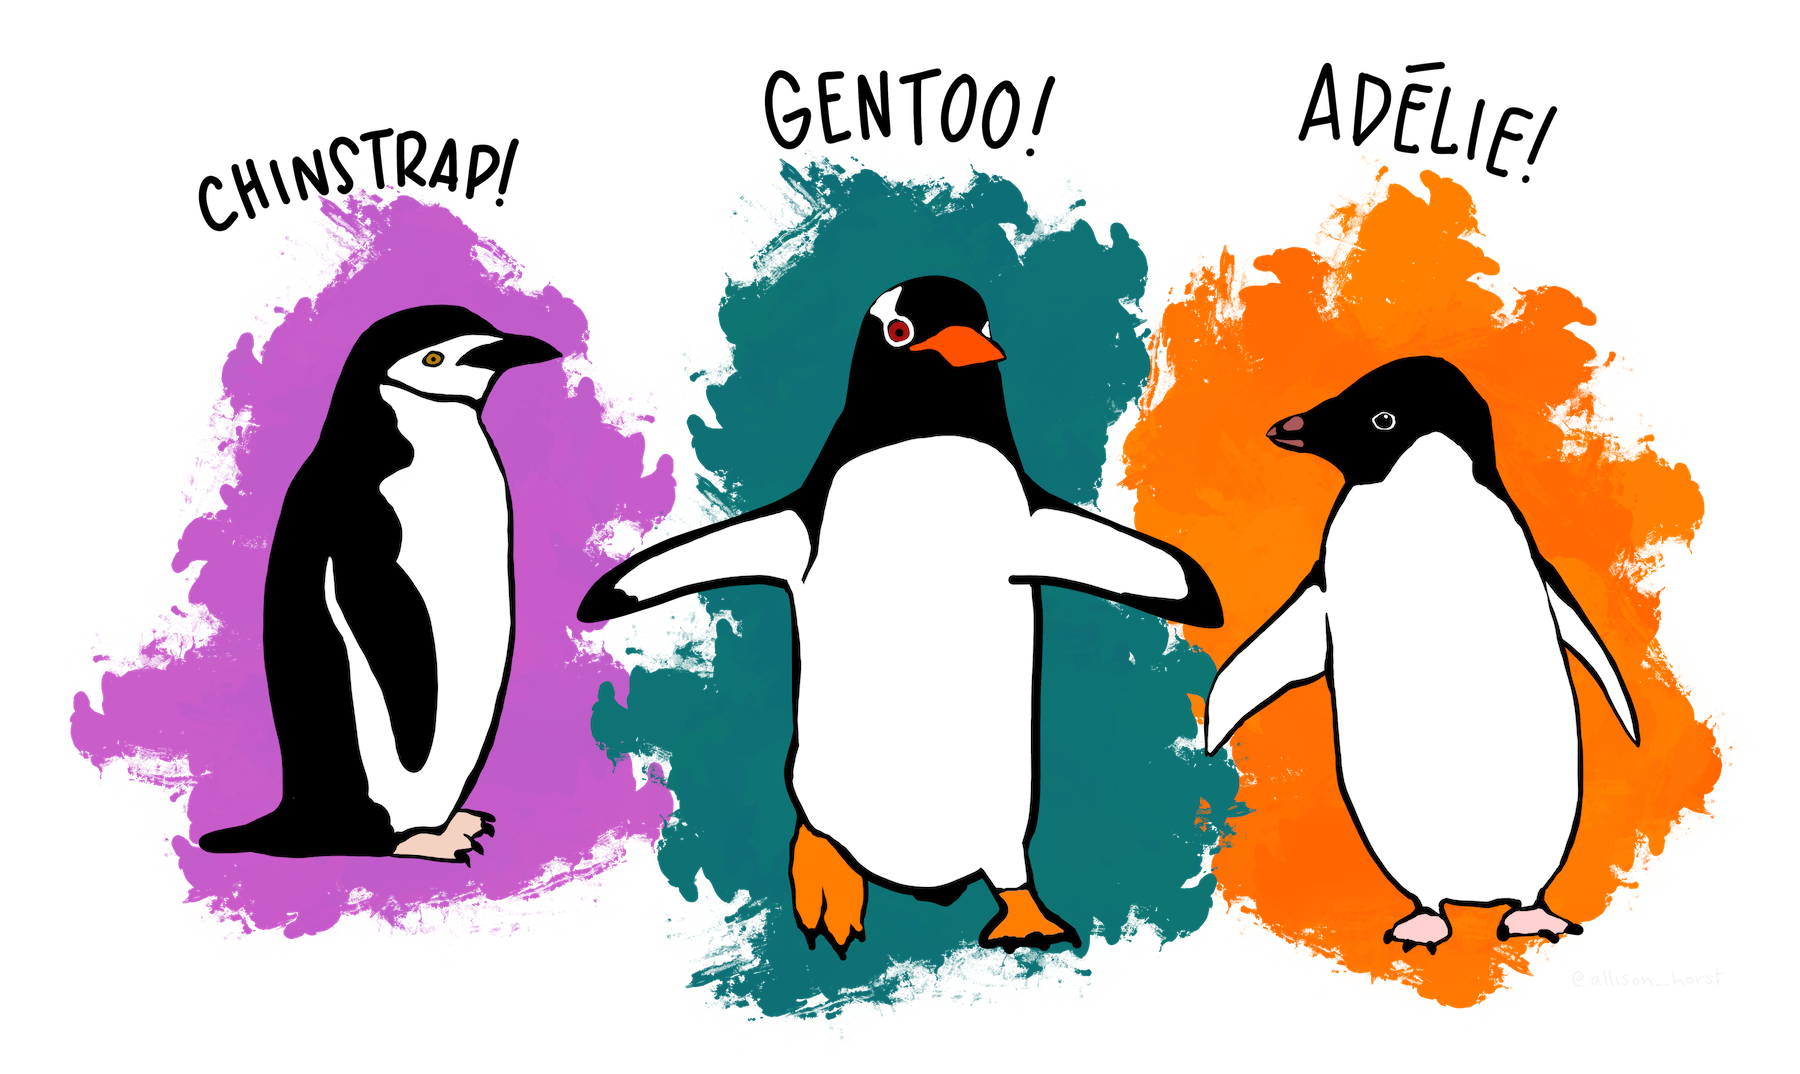
\includegraphics[height=0.52\textheight]{lter_penguins.png}\\[2pt]
    \creditoHorst
  }{%
    \begin{tikzpicture}[scale=0.8]
      \begin{scope}[shift={(-4.2,0)}]  \pingAdelie   \end{scope}
      \begin{scope}[shift={(0,0)}]     \pingChinstrap\end{scope}
      \begin{scope}[shift={(4.2,0)}]   \pingGentoo   \end{scope}
      \node[align=center] at (-4.2,-1.7) {\textbf{Adelia}};
      \node[align=center] at (0,-1.7)    {\textbf{Barbijo}};
      \node[align=center] at (4.2,-1.7)  {\textbf{Juanito}};
    \end{tikzpicture}
  }
  
  \vspace{0.25cm}
  {\small
  \begin{tabular}{@{}lll@{}}
    \textbf{Barbijo} \textit{(P. antarcticus)} & \textbf{Juanito} \textit{(P. papua)} & \textbf{Adelia} \textit{(P. adeliae)}   \\
    {\scriptsize franja negra bajo el mentón} &  {\scriptsize parche blanco sobre los ojos} & {\scriptsize anillo blanco en el ojo}\\
    {\scriptsize 68 individuos}  & {\scriptsize 124 individuos} & {\scriptsize 152 individuos}  \\
  \end{tabular}}
  \end{center}

  \vspace{0.2cm}
  {\footnotesize Tres especies, tres islas, cuatro medidas por individuo. Un conjunto pequeño, pero que nos ayudará a ilustrar los conceptos de casi todo el curso.}
\end{frame}
% ============================================================
\begin{frame}{¿Qué es exactamente lo que se mide?}
  \begin{columns}[T]
    \begin{column}{0.52\textwidth}
      \centering
      \IfFileExists{figuras/culmen_depth.png}{%
        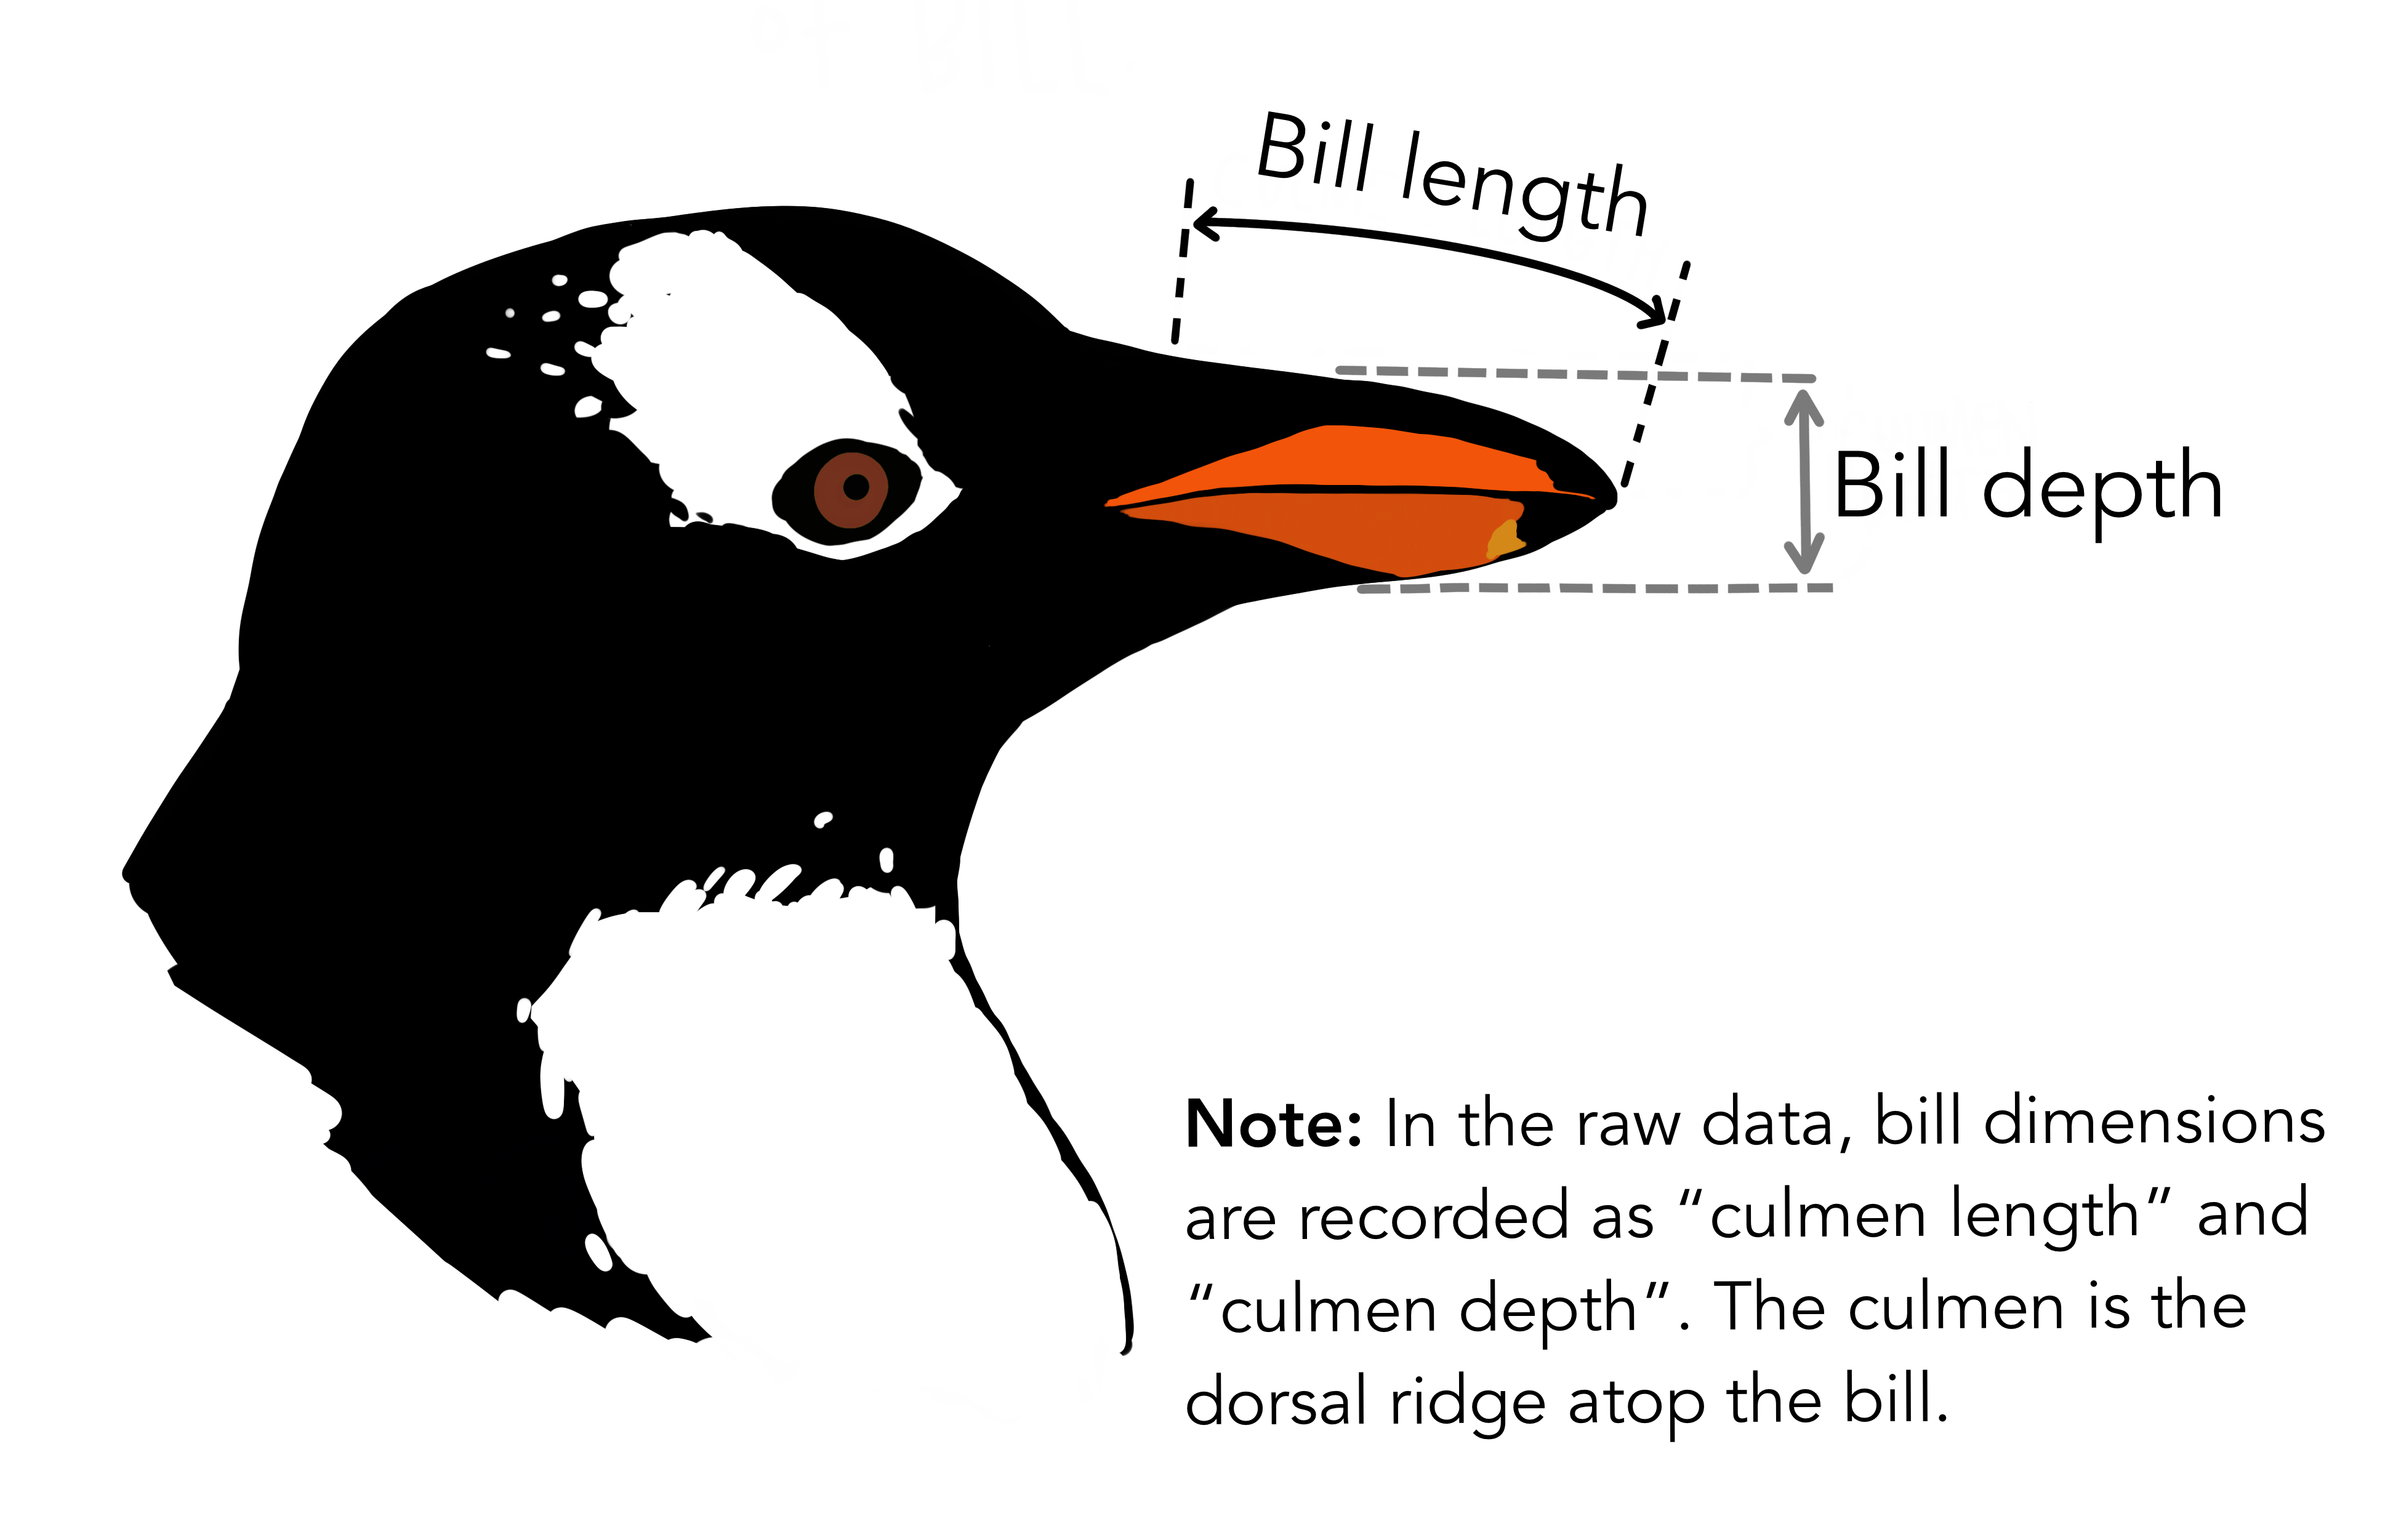
\includegraphics[width=\textwidth]{culmen_depth.png}\\[2pt]
        \creditoHorst
      }{%
        {\color{grisT}\small[Figura de las dimensiones del pico]}
      }
    \end{column}
    \begin{column}{0.44\textwidth}
      \vspace{0.4cm}
      Cada pingüino aporta cuatro medidas:
      \begin{itemize}
        \item Largo del pico (mm)
        \item Profundidad del pico (mm)
        \item Largo de la aleta (mm)
        \item Masa corporal (g)
      \end{itemize}
      \vspace{0.3cm}
      \destaca{\small Vale la pena notar que \textbf{definir \emph{cómo} se mide una variable
      es parte del trabajo estadístico}. Si dos personas miden el pico de forma distinta,
      los datos no son comparables.}
    \end{column}
  \end{columns}
\end{frame}
% ============================================================
\begin{frame}{¿De dónde salieron estos datos?}
  % Prioridad de imágenes:
  %  1) fig1-palmer.png  = Figura 1 del artículo original (CC-BY, ver notas al final)
  %  2) r-mapa-palmer.png = mapa generado en R con las coordenadas publicadas
  %  3) mensaje de respaldo
  \centering
  \IfFileExists{figuras/fig1-palmer.png}{%
    \includegraphics[height=0.66\textheight]{fig1-palmer.png}\\[2pt]
    {\tiny\color{grisT} Gorman KB, Williams TD, Fraser WR (2014), PLoS ONE 9(3):e90081, Fig.~1.
    Reproducida bajo licencia CC-BY.}
  }{%
    \IfFileExists{figuras/r-mapa-palmer.png}{%
      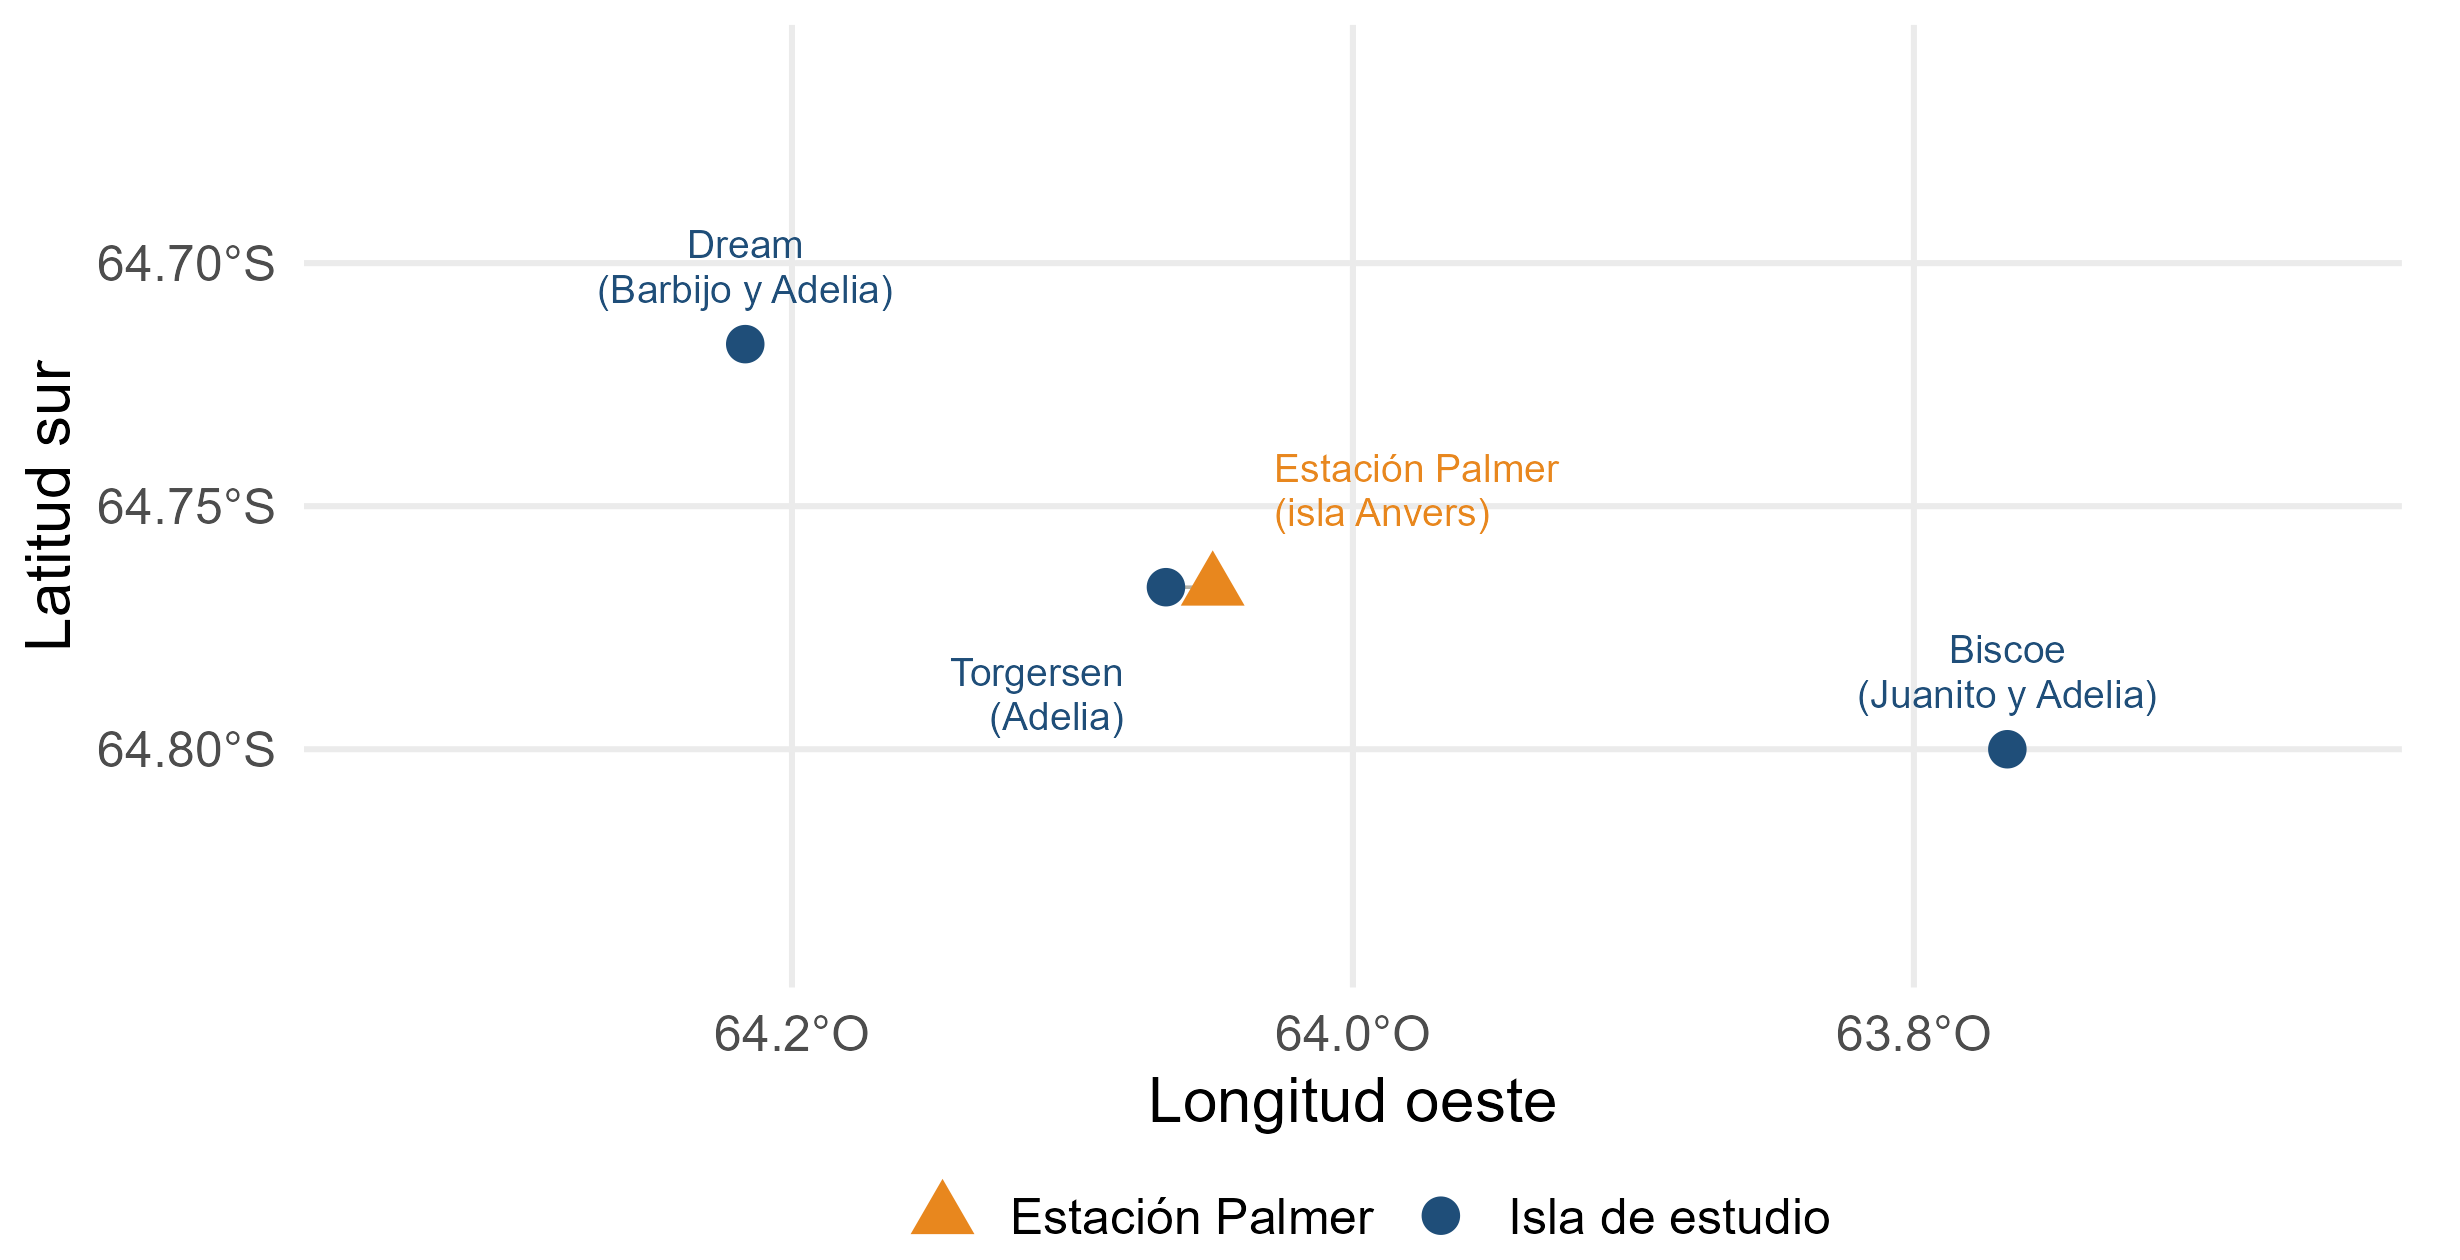
\includegraphics[height=0.66\textheight]{r-mapa-palmer.png}\\[2pt]
      {\tiny\color{grisT}\small Mapa del archipiélago Palmer}
    }{%
      {\color{grisT}\small[Mapa del archipiélago Palmer]}
    }%
  }
  
  \vspace{0.15cm}
  {\footnotesize Archipiélago Palmer, al oeste de la Península Antártica.\\ Las tres islas
  de estudio están a pocos kilómetros de la estación Palmer, en la isla Anvers.}
\end{frame}
\begin{frame}{La estación Palmer}
  \begin{columns}[T]
    \begin{column}{0.55\textwidth}
      Estación de investigación de Estados Unidos en la \textbf{isla Anvers}
      ($64^\circ 46'$S, $64^\circ 03'$O), al oeste de la Península Antártica.
      \vspace{0.3cm}
      \begin{itemize}
        \item Forma parte de la red \textbf{LTER} (\textit{Long Term Ecological Research}):
          proyectos de monitoreo que duran décadas
        \item Los datos se tomaron en tres \textbf{temporadas de campo}: 2007/08, 2008/09 y 2009/10.
          Se escriben con dos años porque el verano austral va de noviembre a febrero, es decir,
          cruza el fin de año
        \item Investigación de la Dra.~Kristen Gorman, con permisos del Acta de Conservación
          Antártica y de comités de cuidado animal
      \end{itemize}
    \end{column}
    \begin{column}{0.42\textwidth}
      \destaca{\small Tres veranos de trabajo de campo en la Antártida para obtener
      344 renglones de datos.

      \vspace{0.25cm}
      \textbf{Vale la pena tenerlo presente cada vez que abramos este archivo. Detrás de cada
      renglón hubo alguien en el hielo, con un calibrador en la mano.}}
    \end{column}
  \end{columns}
\end{frame}
% ============================================================
\begin{frame}{Extracto del archivo real}
  \centering
  {\scriptsize
  \begin{tabular}{@{}rlllrrrrl@{}}
    \toprule
    & \textbf{species} & \textbf{island} & \textbf{sex} & \textbf{bill\_length} & \textbf{bill\_depth} & \textbf{flipper} & \textbf{body\_mass} & \textbf{year} \\
    & & & & {\tiny\color{grisT}mm} & {\tiny\color{grisT}mm} & {\tiny\color{grisT}mm} & {\tiny\color{grisT}gramos} & \\
    \midrule
    1 & Adelie & Torgersen & male   & 39.1 & 18.7 & 181 & 3750 & 2007 \\
    2 & Adelie & Torgersen & female & 39.5 & 17.4 & 186 & 3800 & 2007 \\
    3 & Adelie & Torgersen & female & 40.3 & 18.0 & 195 & 3250 & 2007 \\
    4 & Adelie & Torgersen & \textcolor{rojoAc}{NA} & \textcolor{rojoAc}{NA} & \textcolor{rojoAc}{NA} & \textcolor{rojoAc}{NA} & \textcolor{rojoAc}{NA} & 2007 \\
    5 & Adelie & Torgersen & female & 36.7 & 19.3 & 193 & 3450 & 2007 \\
    6 & Adelie & Torgersen & male   & 39.3 & 20.6 & 190 & 3650 & 2007 \\
    \multicolumn{9}{c}{\textcolor{grisT}{\textit{... 338 renglones más}}} \\
    \bottomrule
  \end{tabular}}

  \vspace{0.45cm}
  \raggedright
  \destaca{Contiene 344 renglones y 8 columnas. Los nombres están en inglés porque así vienen
  en el paquete, y así los vamos a escribir en R. Las tres medidas de longitud están en
  milímetros y la masa en gramos.

  \vspace{0.2cm}
  Nótese el renglón 4: casi todo \textcolor{rojoAc}{\texttt{NA}}. Ese pingüino se registró
  pero no se le pudo medir. Más adelante veremos por qué, y cómo trabajar con esos casos.}
\end{frame}
% ============================================================
\begin{frame}{Diccionario del conjunto de datos}
  Todo conjunto de datos serio viene con su \textbf{diccionario}, donde se indica qué significa cada
  columna, de qué tipo es y en qué unidades está medida.
  
  \vspace{0.3cm}
  \centering
  {\scriptsize
  \begin{tabular}{@{}llllc@{}}
    \toprule
    \textbf{Variable} & \textbf{Significado} & \textbf{Tipo} & \textbf{Valores o unidad} & \textbf{Faltantes} \\
    \midrule
    \texttt{species}    & Especie del pingüino & Categórica nominal & Adelie, Chinstrap, Gentoo & 0 \\
    \texttt{island}     & Isla donde se observó & Categórica nominal & Biscoe, Dream, Torgersen & 0 \\
    \texttt{bill\_length\_mm} & Largo del culmen (pico) & Cuantitativa continua & milímetros & 2 \\
    \texttt{bill\_depth\_mm}  & Profundidad del culmen & Cuantitativa continua & milímetros & 2 \\
    \texttt{flipper\_length\_mm} & Largo de la aleta derecha & Cuantitativa discreta & milímetros & 2 \\
    \texttt{body\_mass\_g}    & Masa corporal & Cuantitativa discreta & gramos & 2 \\
    \texttt{sex}        & Sexo, determinado por ADN & Categórica nominal & female, male & 11 \\
    \texttt{year}       & Temporada de estudio & Categórica ordinal & 2007, 2008, 2009 & 0 \\
    \bottomrule
  \end{tabular}}
  \vspace{0.4cm}
  \raggedright
  \destaca{\small Nótese que \texttt{year} es un número pero funciona como \textbf{etiqueta}:
  promediar años no tiene sentido. Y que hay más faltantes en \texttt{sex} (11) que en las
  medidas (2): a esos once no se les pudo determinar el sexo en el laboratorio.
  
  \vspace{0.2cm}
  El diccionario completo del conjunto está en el libro, junto con los de los otros
  conjuntos del curso. \textbf{Consultar del diccionario es el primer paso de cualquier análisis.}}
\end{frame}
% ============================================================
\begin{frame}{¿Qué preguntas motivaron todo este trabajo?}
  Nadie va tres veranos a la Antártida sin una pregunta. Las del estudio original
  fueron tres.

  \vspace{0.15cm}
  \centering
  {\small
  \begin{tabular}{@{}p{7.2cm}p{4.8cm}@{}}
    \toprule
    \textbf{Pregunta} & \textbf{Técnica que la resuelve} \\
    \midrule
    \textcolor[HTML]{1F4E79}{$\bullet$} ¿Existe \textbf{dimorfismo sexual} en el tamaño
    corporal de estas tres especies? ¿Machos y hembras difieren en tamaño? &
      Prueba $t$ para dos grupos independientes {\scriptsize\color{grisT}(unidad 8)} \\
    \textcolor[HTML]{1F4E79}{$\bullet$} ¿Se puede \textbf{determinar el sexo} de un
    pingüino a partir de sus medidas corporales, sin análisis de ADN? &
      Clasificación con regresión logística o análisis discriminante
      {\scriptsize\color{rojoAc}(fuera del temario)} \\
    \textcolor[HTML]{1F4E79}{$\bullet$} ¿Está relacionada la variabilidad ambiental
    (el \textbf{hielo marino} de cada invierno) con las diferencias de alimentación
    entre machos y hembras? &
      Correlación y regresión {\scriptsize\color{grisT}(unidades 3 y 11)}, sobre
      variables que \textcolor{rojoAc}{no están en nuestra tabla} \\
    \bottomrule
  \end{tabular}}

  \vspace{0.15cm}
  \raggedright
  \destaca{\small Las preguntas explican cada decisión del diseño. Por eso se midió a
  \textbf{los dos} miembros de cada pareja (para comparar sexos), por eso se determinó el
  sexo por \textbf{ADN} (para tener la respuesta correcta con la que comparar), y por eso
  se midieron \textbf{cuatro dimensiones} corporales (para ver cuáles predicen el sexo).

  \vspace{3mm}
  \textbf{Qué preguntas se pueden responder depende de qué variables se midieron,} no de
  qué técnica se conoce. Si la variable no está en la tabla, no podemos contar con ella.}
\end{frame}
% ------------------------------------------------------------
%  DOS DIAPOSITIVAS OPCIONALES, DESACTIVADAS.
%  Traducen las tres preguntas de Palmer a renglones del mapa de decisión.
%  Se dejaron apagadas para no mover la numeración del resto.
%  Para encenderlas, seleccionar el bloque de abajo y quitarle el comentario.
%  En Overleaf, Ctrl + / hace las dos cosas.
% ------------------------------------------------------------
%  \begin{frame}{Cómo se traduce una pregunta en una técnica}
%    Ante cualquier pregunta que traiga alguien del área, un estadístico hace tres
%    preguntas antes de mirar el mapa de decisión:
%
%    \vspace{0.3cm}
%    \begin{enumerate}
%      \item ¿Cuál es la variable \textbf{respuesta}, y de qué \textbf{tipo} es?
%        {\small (cuantitativa o categórica)}
%        \vspace{0.15cm}
%      \item ¿Cuál es la variable \textbf{explicativa}, y de qué tipo? Si es
%        categórica, ¿\textbf{cuántos niveles} tiene?
%        \vspace{0.15cm}
%      \item ¿\textbf{Cómo se obtuvieron} los datos? ¿Grupos independientes, o dos
%        medidas del \emph{mismo} individuo?
%    \end{enumerate}
%
%    \vspace{0.35cm}
%    Las dos primeras eligen el renglón. La tercera decide entre dos renglones que se
%    parecen. Y de fondo hay una cuarta: ¿la pregunta es de \textbf{diferencia}, de
%    \textbf{relación} o de \textbf{predicción}?
%
%    \vspace{0.3cm}
%    \destaca{El mapa de decisión \textbf{no se consulta con las palabras del
%    problema, sino con los tipos de variable}. Traducir de un lenguaje al otro es
%    la habilidad que se practica todo el semestre.}
%  \end{frame}
%  % ============================================================
%  \begin{frame}{Las tres preguntas de Palmer, traducidas}
%    \begin{center}
%    {\scriptsize
%    \begin{tabular}{@{}p{4.3cm}p{4.5cm}p{3.6cm}@{}}
%      \toprule
%      \textbf{Lo que dice quien trae el problema} & \textbf{Lo que oye un estadístico} &
%      \textbf{Renglón del mapa} \\
%      \midrule
%      ¿Difieren machos y hembras en tamaño? &
%        Cuantitativa contra categórica de \textbf{2 niveles}, grupos independientes &
%        Dos grupos independientes {\scriptsize\color{grisT}(unidad 8)} \\
%      \dots y si fueran los dos del \emph{mismo nido} &
%        Cuantitativa, \textbf{dos medidas del mismo par} &
%        Datos pareados {\scriptsize\color{grisT}(unidad 8)} \\
%      ¿Y en cuál especie la diferencia es mayor? &
%        Cuantitativa contra \textbf{dos} categóricas: es una \textbf{interacción} &
%        \textcolor{rojoAc}{No está en el mapa: ANOVA de dos factores} \\
%      ¿Se puede adivinar el sexo a partir de las medidas? &
%        La respuesta ahora es \textbf{categórica}, con explicativas cuantitativas &
%        \textcolor{rojoAc}{No está en el mapa: regresión logística} \\
%      ¿Se relacionan el hielo marino y la alimentación? &
%        Dos cuantitativas &
%        Correlación {\scriptsize\color{grisT}(unidad 3)} y \Rc{lm()}
%        {\scriptsize\color{grisT}(unidad 11)} \\
%      \bottomrule
%    \end{tabular}}
%    \end{center}
%
%    \vspace{0.3cm}
%    \raggedright
%    \destaca{\small Dos observaciones que valen todo el curso.
%
%    \vspace{0.15cm}
%    \textbf{El renglón 1 y el 2 son la misma pregunta con datos distintos.} El estudio
%    midió al macho \emph{y} a la hembra del mismo nido. Eso es pareado, y la prueba
%    pareada detecta diferencias más pequeñas. Pero nuestra tabla no trae el
%    identificador del nido, así que perdimos esa ventaja.
%
%    \vspace{0.15cm}
%    \textbf{El renglón 1 y el 4 usan las mismas dos variables, con los papeles
%    invertidos.} ``¿La masa depende del sexo?'' y ``¿puedo adivinar el sexo si conozco
%    la masa?'' no son la misma pregunta, y no se contestan con la misma técnica.}
%  \end{frame}
%
% ------------------------------------------------------------
% ============================================================
\begin{frame}{¿Qué más le podemos preguntar a estos datos?}
  \centering
  {\small
  \begin{tabular}{@{}p{7.2cm}p{4.8cm}@{}}
    \toprule
    \textbf{Pregunta} & \textbf{Técnica o medida que la resuelve} \\
    \midrule
    \textcolor[HTML]{1F4E79}{$\bullet$} ¿Cuánto pesa un pingüino típico? ¿Qué tan parecidos son entre sí? &
      Media, mediana, desviación estándar {\scriptsize\color{grisT}(unidades 1--2)} \\
    \textcolor[HTML]{1F4E79}{$\bullet$} ¿Los pingüinos con aletas más largas pesan más? &
      Coeficiente de correlación y recta de regresión {\scriptsize\color{grisT}(unidad 3)} \\
    \textcolor[HTML]{1F4E79}{$\bullet$} Los Juanito de esta muestra pesaron más que los Adelia. ¿Pasa lo mismo en \emph{toda} la población, o fue casualidad de estos 344? &
      Intervalo de confianza y prueba $t$ para dos medias {\scriptsize\color{grisT}(unidades 7--8)} \\
    \textcolor[HTML]{1F4E79}{$\bullet$} ¿Difieren las \emph{tres} especies en el largo del pico, o solo alguna? &
      ANOVA y comparaciones post-hoc {\scriptsize\color{grisT}(unidad 10)} \\
    \textcolor[HTML]{1F4E79}{$\bullet$} ¿Difiere la proporción de machos entre especies? &
      Prueba ji-cuadrada en tabla de contingencia {\scriptsize\color{grisT}(unidad 9)} \\
    \textcolor[HTML]{1F4E79}{$\bullet$} ¿Se puede predecir la masa a partir de la aleta, y con cuánto error? &
      Regresión lineal, $R^2$ e intervalos de predicción {\scriptsize\color{grisT}(unidad 11)} \\
    \bottomrule
  \end{tabular}}
  \vspace{2mm}
  \destaca{\small Cada tipo de pregunta necesita una técnica distinta, de eso trata el curso: \textbf{describir
  lo que vemos}, y hacer \textbf{inferencias, es decir afirmar algo sobre toda la población habiendo visto solo una muestra, y decir con cuánta confianza lo afirmamos.}}
\end{frame}
% ============================================================
\begin{frame}{El diseño del estudio}
  \destaca{Las acciones llevadas a cabo por los investigadores para registrar los datos no fueron improvisadas. Los nidos se marcaron \textbf{antes} de que las hembras pusieran el primer huevo, y se monitorearon de forma constante. Esto es, \textbf{había un plan antes de obtener los datos}.}
  \vspace{0.4cm}
  \centering
  {\small
  \begin{tabular}{@{}lccc@{}}
    \toprule
    \textbf{Especie} & \textbf{Nidos por temporada} & \textbf{Islas} & \textbf{Distribución} \\
    \midrule
    Adelia  & 30 & Biscoe, Dream y Torgersen & 10 nidos en cada isla \\
    Juanito & 30 & Biscoe & todos en la misma isla \\
    Barbijo & 15 & Dream & todos en la misma isla \\
    \bottomrule
  \end{tabular}}

  \vspace{0.5cm}
  \raggedright
  {\footnotesize ¿Por qué los Barbijo son la mitad? Porque en las colonias de Dream
  anidaban menos individuos. El tamaño de muestra no siempre lo decide quien investiga:
  a veces lo decide la naturaleza.}
\end{frame}
% ============================================================
\begin{frame}{El protocolo de medición}
  Cada vez que un nido llegaba a la etapa de \textbf{un huevo}, se capturaba a
  \textbf{los dos adultos} de la pareja y se registraba:
    \vspace{0.35cm}

    \centering
    {\small
  \begin{tabular}{@{}lll@{}}
    \toprule
    \textbf{Medida} & \textbf{Instrumento} & \textbf{Precisión} \\
    \midrule
    Largo y profundidad del pico & Calibrador de carátula & $\pm 0.1$ mm \\
    Largo de la aleta derecha & Regla & $\pm 1$ mm \\
    Masa corporal & Balanza de resorte y bolsa & $\pm 25$ o $\pm 50$ g \\
    Sexo & Análisis de ADN (PCR) & --- \\
    \bottomrule
  \end{tabular}}

  \vspace{0.5cm}
  \raggedright
  \destaca{Tres cosas que un estadístico nota de inmediato:
  \vspace{0.2cm}
  \textbf{Siempre la aleta derecha}, nunca ``una aleta''. El instrumento y su precisión
  están \textbf{escritos en el protocolo}. Y el sexo se determinó por \textbf{ADN}, no
  a simple vista.}
\end{frame}
% ============================================================
\begin{frame}{Los controles del diseño}
  \begin{columns}[T]
    \begin{column}{0.48\textwidth}
      \textbf{Todos en la misma etapa}\\[3pt]
      {\small Se midió a todos los adultos exactamente en la etapa de \emph{un huevo}.
      La masa de un pingüino cambia muchísimo a lo largo de la reproducción, medirlos
      en momentos distintos habría hecho incomparables los datos.}
      
      \vspace{0.35cm}
      \textbf{La pareja completa}\\[3pt]
      {\small De cada nido se midió al macho \emph{y} a la hembra. En el estudio original
      los datos son \textbf{pareados}, y eso permite comparaciones más finas. Nuestra
      tabla, en cambio, no trae el identificador del nido, así que esa ventaja se perdió
      al simplificarla.}
    \end{column}
    \begin{column}{0.48\textwidth}
      \textbf{Seguimiento posterior}\\[3pt]
      {\small Después de manipularlos, se siguió vigilando cada nido para confirmar
      que la pareja completara su nidada de dos huevos.}
      \vspace{0.35cm}
      \destaca{\small Esto es \textbf{control} en el sentido técnico: \textbf{mantener constante
      todo lo que no se está estudiando, para que las diferencias observadas se deban
      a lo que sí interesa}.% (unidad 5).
 }
    \end{column}
  \end{columns}
\end{frame}
% ============================================================
\begin{frame}{Los datos faltantes: \texttt{NA}}
  Del plan original no todo se pudo cumplir:
  \vspace{0.35cm}
  \begin{itemize}
    \item Hubo días en que \textbf{el clima impidió llegar} a las colonias. Algunos nidos
      no se muestrearon porque, al volver, la pareja ya había completado la nidada.
    \item Algunas parejas se \textbf{excluyeron del análisis} porque nunca se observó el
      segundo huevo, probablemente depredado por la \textbf{skúa café}. Sin ese dato no
      había certeza de que los adultos estuvieran exactamente en la etapa de un huevo.
  \end{itemize}

  \vspace{0.4cm}
  \destaca{Por eso el archivo tiene celdas vacías (\texttt{NA}) y por eso los tamaños
  finales quedaron desiguales: \textbf{152} Adelia, \textbf{124} Juanito y \textbf{68} Barbijo.

  \vspace{0.25cm}
  Los datos faltantes casi nunca faltan al azar: \textbf{tienen una causa}. Aquí fueron
  el clima y un ave depredadora. \textbf{Preguntar por qué falta un dato es parte del análisis, así como tomar la decisión de qué hacer con dichos faltantes}.}
\end{frame}
% ============================================================
\begin{frame}{Entender el contexto del problema y el origen de los datos IMPORTA}
  Al contar cuántos pingüinos de cada especie hay en cada isla, resulta esta tabla
  (una \textbf{tabla de contingencia}):

  \centering
  {\small
  \begin{tabular}{@{}lrrrr@{}}
    \toprule
    & \textbf{Biscoe} & \textbf{Dream} & \textbf{Torgersen} & \textbf{Total} \\
    \midrule
    Adelia  & 44 & 56 & 52 & 152 \\
    Barbijo & 0  & 68 & 0  & 68 \\
    Juanito & 124 & 0 & 0  & 124 \\
    \midrule
    \textbf{Total} & 168 & 124 & 52 & 344 \\
    \bottomrule
  \end{tabular}}

  \vspace{0.3cm}
  \raggedright
  En la unidad 9 veremos una prueba para decidir si dos variables categóricas están
  \textbf{asociadas}. Aplicada aquí, saldría una \textbf{asociación fuerte}, pero es debido a los ceros, que hacen que \texttt{especie} e \texttt{isla} ``parezcan`` íntimamente ligadas. Sin embargo, concluir ``\emph{descubrimos que la especie depende de la isla}'' \textbf{¡sería un error!}. Esos ceros no son un hallazgo sobre la naturaleza. Son consecuencia
  del \textbf{diseño del muestreo}. \textbf{Los Juanito se buscaron únicamente en Biscoe y los
  Barbijo únicamente en Dream, porque ahí están sus colonias}.

  \vspace{0.2cm}
  \destaca{
  Por esto \textbf{es muy importante entender el contexto del problema} aunque no seamos del área,  \textbf{y comprender cómo se recolectaron los datos}.}
\end{frame}

% ============================================================
\section{Introducción a R y RStudio}
% ---------- bloque: R y RStudio ----------
%  Una clase completa dedicada al software, antes de empezar la Unidad 1.
%  El razonamiento: si R se introduce a cuentagotas (una línea copiada del
%  pizarrón cada día), nunca se vuelve una herramienta propia. Conviene invertir
%  una sesión entera para que después el software no compita con la estadística
%  por la atención del grupo.
%  Requisito: todos con su computadora y la instalación hecha, que se dejó de tarea
%  al presentar el curso.
%  La diapositiva siguiente, la de comprobar la instalación, conviene mostrarla al
%  final de la clase anterior si sobra tiempo: así los problemas de instalación aparecen
%  un día antes y no al arrancar esta sesión.
\begin{frame}[plain]
  \hojaSesion{Introducción a R y RStudio}{%
  Reconocer la interfaz y saber dónde se escribe cada cosa. Ejecutar código, usar
  R como calculadora y ver que además es un lenguaje de programación. Cargar el conjunto
  \texttt{penguins} desde su librería, explorarlo y manipular la tabla con R base.}
\end{frame}

% ============================================================
\begin{frame}{Las cuatro ventanas de RStudio}

  \begin{center}
  \IfFileExists{figuras/rstudio-ventanas.png}{%
    \includegraphics[height=0.60\textheight]{rstudio-ventanas.png}
  }{%
  \begin{tikzpicture}[scale=0.82,every node/.style={align=center}]
    % fondos
    \fill[azulClaro] (0.06,3.06) rectangle (7.44,5.94);
    \fill[azulClaro!45] (0.06,0.06) rectangle (7.44,2.94);
    \fill[azulClaro!45] (7.56,3.06) rectangle (12.94,5.94);
    \fill[azulClaro!45] (7.56,0.06) rectangle (12.94,2.94);
    % marcos
    \draw[grisT,thick] (0,0) rectangle (13,6);
    \draw[grisT,thick] (7.5,0) -- (7.5,6);
    \draw[grisT,thick] (0,3) -- (13,3);
    % contenido
    \node[font=\small\bfseries,text=azulUS] at (3.75,5.45) {1. Editor (\emph{Source})};
    \node[font=\scriptsize,text width=6.6cm] at (3.75,4.15)
      {Aquí se escribe el código \textbf{que se guarda}: los archivos \texttt{.R} y
       \texttt{.qmd}.\\[2pt] Con \textbf{Ctrl + Enter} se ejecuta \\[2pt] rápidamente una instrucción.};
    \node[font=\small\bfseries,text=azulUS] at (3.75,2.5) {2. Consola};
    \node[font=\scriptsize,text width=6.6cm] at (3.75,1.3)
      {R dentro de RStudio. \\[2pt] Aquí aparecen los resultados. Lo que se teclea
       directamente aquí \textbf{no queda guardado}.\\[2pt]
       Junto a ella hay una pestaña \textbf{Terminal}, que \emph{no} es R.};
    \node[font=\small\bfseries,text=azulUS] at (10.25,5.45) {3. Environment};
    \node[font=\scriptsize,text width=4.8cm] at (10.25,4.2)
      {Contiene los \textbf{objetos que existen} en esta sesión: tablas, vectores, funciones.\\[2pt]
       Si algo no aparece aquí, R no lo conoce.};
    \node[font=\small\bfseries,text=azulUS] at (10.25,2.5) {4. Files · Plots · Help};
    \node[font=\scriptsize,text width=4.8cm] at (10.25,1.3)
      {Los archivos de la carpeta, las gráficas que se producen, los paquetes
       instalados y la ayuda.};
  \end{tikzpicture}}
\end{center}
  
  \vspace{0.2cm}
  {\footnotesize Si al abrir RStudio faltara alguna ventana:
  \textbf{View $\rightarrow$ Panes $\rightarrow$ Show All Panes}.}
\end{frame}
% ============================================================
\begin{frame}{Consola, script y terminal}
  \centering
  {\small
  \begin{tabular}{@{}p{2.6cm}p{4.9cm}p{4.9cm}@{}}
    \toprule
    \textbf{Dónde} & \textbf{Qué es} & \textbf{Cuándo se usa} \\
    \midrule
    \textbf{Consola} & El intérprete de R esperando una orden. Lo que se escribe
      se ejecuta y se pierde &
      Para probar algo rápido: ver una tabla, revisar un valor, consultar la ayuda \\
    \textbf{Script}  {\scriptsize(archivo \texttt{.R})} &
      Un archivo de texto con código, que se guarda &
      Para todo lo que se va a entregar o repetir. \textbf{Aquí se trabaja} \\
    \textbf{Terminal} & La línea de comandos \textbf{del sistema operativo}, no de R. &
      Para \texttt{git}, para moverse entre carpetas, o para arrancar R sin RStudio
      escribiendo \texttt{R} \\
    \bottomrule
  \end{tabular}}
  
  \vspace{0.5cm}
  \raggedright
  \destaca{Para el curso se sugiere \textbf{escribir en el script}, ya que un análisis que solo existe en la consola no se guarda, así que no podrán recuperarlo la próxima vez que abran RStudio. No es reproducible.}
\end{frame}

% ============================================================
\begin{frame}[fragile]{R como calculadora}
\begin{lstlisting}
2 + 3 * 4        # 14, la jerarquia de operaciones es la usual
(2 + 3) * 4      # 20
7 / 2            # 3.5
7 %/% 2          # 3    division entera
7 %% 2           # 1    residuo
2^10             # 1024
sqrt(2)          # 1.414214
log(100, base = 10)   # 2
round(pi, 3)     # 3.142
\end{lstlisting}

  \vspace{0.25cm}
  \destaca{\small  Con la \textbf{flecha hacia arriba} se recupera el último comando, y con
  \textbf{Tab} R completa el nombre de una función.}
\end{frame}

% ============================================================
\begin{frame}[fragile]{R también es un lenguaje de programación}
\begin{lstlisting}
a <- 3; b <- 10    # <- es el simbolo de asignacion

x <- c(1, 2, 3)    # concatenar valores para crear un vector
x / 1000           # opera sobre TODO el vector, sin ciclo
x[1]               # extraer el primer elemento 

y <- c(10, 20, 30, 40, 50)
x + y              # tiene sentido la suma aunque los vectores no tengan igual longitud, el vector corto se "recicla"
\end{lstlisting}

  \vspace{0.2cm}
  \destaca{\small Precauciones para quienes vienen de otro lenguaje:
  \begin{itemize}
      \item los índices \textbf{empiezan en 1}
      \item casi ninguna operación necesita un ciclo
  porque las funciones \textbf{trabajan sobre vectores completos}
  \item \textbf{el reciclaje} (como en el ejemplo \texttt{x + y}) 
  puede ser una fuente de errores difíciles de ver.
  \end{itemize} 
  
  \vspace{0.2cm}
  Se pueden definir funciones, como es de esperarse:
  \Rc{promedio <- function(x) sum(x) / length(x)}. No profundizaremos en eso, pues
  el objetivo del curso es \textbf{usar} R para analizar datos.}
\end{frame}



% ============================================================



\begin{frame}[fragile]{Cargar datos que vienen en una librería: \texttt{penguins}}

Instalamos el paquete en nuestra máquina: 
\begin{lstlisting}
install.packages("palmerpenguins")
\end{lstlisting}

\vspace{4mm}
Cargamos la librería a la sesión actual:
\begin{lstlisting}
library(palmerpenguins)
\end{lstlisting}

  \vspace{0.4cm}
  \destaca{\small   Un paquete se \textbf{instala una sola vez} en la computadora, pero se \textbf{carga con \Rc{library()} en cada sesión} de trabajo. Si cerramos el programa, la próxima vez que ocupemos el dataset deberemos volver a cargar la librería.

  \vspace{0.15cm}
  Documentación del paquete y de los datos:
  \href{https://allisonhorst.github.io/palmerpenguins/}{\texttt{allisonhorst.github.io/palmerpenguins}}}
\end{frame}


% ============================================================
\begin{frame}[fragile]{Comandos para exploración de datos}
\begin{lstlisting}
dim(penguins)             # cantidad de renglones y columnas
nrow(penguins); ncol(penguins)   # cada uno por separado
names(penguins)           # los nombres de las columnas
str(penguins)             # tipo de cada columna y primeros valores
summary(penguins)         # resumen numérico de cada columna, con los NA contados
View(penguins)            # abre la tabla completa en una pestana
\end{lstlisting}

  \vspace{0.3cm}
  \destaca{\small Estas líneas son el \textbf{primer contacto con cualquier
  tabla}.  Obsérvese que la instrucción \Rc{summary(penguins)} devuelve un resumen similar al contenido en el diccionario de la base de datos.}
\end{frame}

% ============================================================
\begin{frame}[fragile]{Explorar y manipular tablas con R base}
\begin{lstlisting}
penguins[ , 1]                               # extraer la columna 1 
penguins$body_mass_g                         # extraer columnas por su nombre
penguins[ , 3:6]                             # extraer varias columnas a la vez (de la 3 a la 6)
penguins[1:10, 6:8]                          # extraer renglones y columnas
penguins[1:5, c("species", "body_mass_g")]   # extraer renglones y columnas por nombre
penguins[penguins$species == "Gentoo", ]     # filtrar renglones
table(penguins$species)                      # contar por categorias
table(penguins$species, penguins$island)     # la tabla de contingencia
mean(penguins$body_mass_g, na.rm = TRUE)     # Media de UNA columna
\end{lstlisting}
% aggregate(body_mass_g ~ species, data = penguins, FUN = mean)

  \vspace{0.25cm}
  \destaca{\small La primera línea es la sintaxis fundamental para \textit{extraer}:
  \textbf{corchete, renglones, coma, columnas, corchete}. Dejar vacío un lado significa ``todas''. También se pueden extraer columnas por su nombre usando el símbolo \$.
  
  \vspace{0.15cm}
    \vspace{0.2cm}
  Nótese que el promedio de algo que incluye un faltante es un faltante (\texttt{NA}). R obliga a decidir
  explícitamente, con \Rc{na.rm = TRUE}, que se van a ignorar.}
\end{frame}

% ============================================================
% ---------- bloque: resumir y manipular tablas ----------
%  Hasta la diapositiva anterior llegó la clase pasada. Esta hoja marca el corte.
%  Ahí se mencionaron de paso apply y dplyr; aquí se retoman con calma.
\begin{frame}[plain]
  \hojaSesion{Continuación con R y RStudio: \\ resumir y manipular tablas}{%
   Resumir por grupos con la familia \texttt{apply} de R base y
  con \texttt{dplyr}, \\ su equivalente moderno. }
\end{frame}


% ============================================================
%  Diapositiva opcional. Se puede omitir sin que nada se rompa después: todo lo
%  que sigue en el curso se resuelve con dplyr. Se incluye porque la familia
%  apply es el idioma del código de R que van a encontrar publicado, y porque a
%  un grupo de computación le interesa ver el estilo funcional del lenguaje.

\begin{frame}[fragile]{Aplicar una función a muchas cosas: la familia \texttt{apply} de R base}

En lugar de escribir un ciclo, le pasamos
  \textbf{una función} (por ejemplo \Rc{mean}) a otra función (de la familia \texttt{apply}) que la aplica sobre cada pedazo. Es el estilo
  funcional del lenguaje, y R lo trae nativamente.
\begin{lstlisting}
sapply(penguins[, 3:6], mean, na.rm = TRUE)   # la media de CADA columna numerica
tapply(penguins$body_mass_g, penguins$species, mean, na.rm = TRUE)
                                              # una media POR especie
\end{lstlisting}
%m <- matrix(1:6, nrow = 2)
%apply(m, 1, sum)     # 9 12      por renglon  (la dimension 1)
%apply(m, 2, sum)     # 3 7 11    por columna  (la dimension 2)
%Reduce(`+`, 1:5)     # 15        R tambien trae Map, Filter y Reduce


  \vspace{0.2cm}
  \destaca{\small
  Nótese que \Rc{tapply} es exactamente \emph{agrupar y resumir} en una línea. Es lo
  que hará \Rc{group\_by() + summarise()} de \texttt{dplyr}, y verlo así ayuda a
  entender qué pasa por detrás. A lo largo del curso usaremos \texttt{dplyr} porque se lee mejor cuando  hay varios pasos encadenados, pero \Rc{sapply} y \Rc{tapply} aparecen en muchas referencias sobre
  código de R.}
\end{frame}


% ============================================================
\begin{frame}[fragile]{Lo mismo, con \texttt{dplyr}}

Instalamos el paquete y cargamos la librería:
\begin{lstlisting}
install.packages("tidyverse")
library(dplyr)
\end{lstlisting}

  \vspace{0.1cm}
  La tarea, resuelta de dos maneras: \textbf{Obtener la masa promedio de los pingüinos
  Gentoo, separada por sexo.}

  \vspace{0.1cm}
  \begin{columns}[T]
    \begin{column}{0.47\textwidth}
      {\footnotesize\textbf{Con R base}}
\begin{lstlisting}
gentoo <- penguins[
  penguins$species == "Gentoo", ]
tapply(gentoo$body_mass_g,
       gentoo$sex,
       mean, na.rm = TRUE)
\end{lstlisting}
    \end{column}
    \begin{column}{0.51\textwidth}
      {\footnotesize\textbf{Con \texttt{dplyr}}}
\begin{lstlisting}
penguins |>
  filter(species == "Gentoo") |>
  group_by(sex) |>
  summarise(masa = mean(body_mass_g,
                        na.rm = TRUE))
\end{lstlisting}
    \end{column}
  \end{columns}

  \vspace{0.2cm}
  \destaca{\small El símbolo \Rc{|>} se llama \textit{pipe} (o tubería) se lee \textbf{``y luego''}. Toma \texttt{penguins},
  \emph{y luego} filtra, \emph{y luego} agrupa, \emph{y luego} resume. La versión de la
  izquierda hay que armarla al revés, guardando antes un resultado intermedio.}
\end{frame}
% ============================================================
\begin{frame}{Los verbos de \texttt{dplyr}}
  \begin{center}
  {\small
  \begin{tabular}{@{}p{3.4cm}p{8.4cm}@{}}
    \toprule
    \textbf{Verbo} & \textbf{Qué hace} \\
    \midrule
    \Rc{filter()}    & Se queda con ciertos renglones \\
    \Rc{select()}    & Se queda con ciertas columnas \\
    \Rc{mutate()}    & Crea una columna nueva \\
    \Rc{arrange()}   & Ordena los renglones \\
    \Rc{summarise()} & Resume la tabla en uno o varios números \\
    \Rc{group\_by()} & Hace que el resumen se calcule por grupo \\
    \bottomrule
  \end{tabular}}
  \end{center}

  \vspace{0.4cm}
  \destaca{Con esos seis y la tubería se resuelve casi todo lo que haremos en el curso.
  La documentación completa, con ejemplos, está en
  \href{https://dplyr.tidyverse.org/}{\texttt{dplyr.tidyverse.org}}}
\end{frame}
% ============================================================
\begin{frame}{Por qué las dos salidas no se ven iguales}
  Los números coinciden. Lo que no coincide es la pantalla, y conviene verlo con calma.

  \vspace{0.3cm}
  \begin{center}
  {\small
  \begin{tabular}{@{}lrrr@{}}
    \toprule
    & \textbf{female} & \textbf{male} & \textbf{sin sexo} \\
    \midrule
    \Rc{tapply()}     & 4679.74 & 5484.84 & \textcolor{rojoAc}{no aparece} \\
    \Rc{summarise()}  & 4679.74 & 5484.84 & 4587.50 \\
    \midrule
    Cuántos son       & 58 & 61 & 5 \\
    \bottomrule
  \end{tabular}}
  \end{center}

  \vspace{0.35cm}
  \destaca{\small Las medias de \texttt{female} y \texttt{male} son \textbf{idénticas}
  por los dos caminos. Lo que cambia son dos cosas:
  \Rc{group\_by()} agrega un tercer renglón con los cinco pingüinos Gentoo a los que no
  se les determinó el sexo, y \Rc{tapply()} los descarta sin avisar. Además
  \texttt{dplyr} redondea al mostrar, así que en pantalla aparece 4680 en lugar de
  4679.74.

  \vspace{0.15cm}
  Que el resumen avise de los casos sin clasificar es una ventaja, no un defecto.}
\end{frame}

% ============================================================
% ---------- bloque: cierre de R ----------
%  La clase anterior llegó hasta la comparación con dplyr, así que el bloque de R
%  se estira una clase más.
\begin{frame}[plain]
  \hojaSesion{Cerramos R y RStudio}{%
  El directorio de trabajo y los tipos de datos. Cómo escribir una tabla en un
  archivo. Cómo leer un archivo propio. Cómo devolverle el tipo \texttt{factor} a una
  columna que llegó como texto. Los errores más comunes. Cerramos con la práctica.}
\end{frame}
% ============================================================
\begin{frame}[fragile]{El directorio de trabajo}
  R busca y guarda archivos a partir de una carpeta, llamada directorio de trabajo:
\begin{lstlisting}
getwd()               # en que carpeta estoy
list.files()          # que hay en ella
list.files("datos")   # que hay en la subcarpeta datos
\end{lstlisting}
  \vspace{0.2cm}
  Se puede cambiar a mano, aunque conviene poco:
\begin{lstlisting}
setwd("C:/Users/yo/Documentos/estadistica")   # con / o con \\, nunca con \
\end{lstlisting}

  \vspace{0.2cm}
  \destaca{\small La forma recomendable es crear un \textbf{Proyecto} de RStudio
  (\textbf{File $\rightarrow$ New Project}). Al abrirlo, el directorio de trabajo
  queda fijado en su carpeta, y entonces basta escribir rutas
  \textbf{relativas} como \Rc{"datos/mi-archivo.csv"}.
  
  \vspace{0.2cm}
  Así el trabajo funciona en cualquier computadora. Un \Rc{setwd()} con la ruta
  personal de quien lo escribió falla en todas las demás máquinas. Es el motivo
  número uno de que un análisis ajeno ``no corra''.}
\end{frame}

% ============================================================
\begin{frame}[fragile]{Tipos de datos en R}
\begin{lstlisting}
class(penguins$body_mass_g)   # "numeric"    un numero
class(penguins$year)          # "integer"    un entero
class(penguins$species)       # "factor"     una categoria
class("Adelie")               # "character"  texto, siempre entre comillas
levels(penguins$species)      # "Adelie" "Chinstrap" "Gentoo"

gentoo <- penguins[penguins$species == "Gentoo", ]
table(gentoo$species)         # Adelie 0, Chinstrap 0, Gentoo 124
\end{lstlisting}

  \vspace{0.25cm}
  \destaca{\small Las dos últimas líneas muestran qué guarda de más un \textbf{factor}.
  En \texttt{gentoo} no quedó ni un solo Adelia, y aun así la tabla sigue reportando esa
  categoría con \textbf{cero casos}, porque el factor recuerda todos los valores
  posibles y no solo los que están presentes.

  \vspace{0.15cm}
  \textbf{Si la columna fuera texto simple, las categorías vacías desaparecerían de la tabla y
  nadie notaría que faltan. Por eso conviene que las variables categóricas sean factor}.}
\end{frame}
% ============================================================
\begin{frame}[fragile]{Los faltantes se contagian}
\begin{lstlisting}
mean(c(3750, NA, 3250))                 # NA        <- se contagia: hay NA y el resultado da NA
mean(c(3750, NA, 3250), na.rm = TRUE)   # 3500
c(3750, NA, 3250) > 3500                # TRUE NA FALSE  <- tambien se contagia

is.na(c(3750, NA, 3250))                # FALSE TRUE FALSE
!is.na(c(3750, NA, 3250))               # TRUE FALSE TRUE
\end{lstlisting}

  \vspace{0.25cm}
  \destaca{\small El promedio de algo que incluye un faltante es un faltante, y una
  comparación contra un faltante también lo es. Es a propósito, R nos obliga a decidir
  qué hacer con lo que falta en lugar de ignorarlo a escondidas.

  \vspace{0.15cm}
  Las dos últimas líneas presentan el signo \Rc{!}, que en R significa \textbf{negación}
  y se lee ``no''. \Rc{is.na(x)} pregunta si cada valor es faltante, y \Rc{!is.na(x)}
  pregunta lo contrario. Así, \Rc{na.rm = TRUE} sirve al resumir y \Rc{!is.na()} sirve
  al filtrar.}
\end{frame}


% ============================================================
\begin{frame}[fragile]{Cargar datos desde un archivo propio}
  Escribamos en un archivo la tabla \texttt{penguins}:
\begin{lstlisting}
write.csv(penguins, "mis-pinguinos.csv", row.names = FALSE)
\end{lstlisting}

\vspace{0.15cm}
Ahora cargamos a la sesión el archivo recién creado, y comprobamos que es como el original:
\begin{lstlisting}
mios <- read.csv("mis-pinguinos.csv")
dim(mios); names(mios); str(mios)
\end{lstlisting}

  \vspace{0.15cm}
  \destaca{\small Si devuelve \Rc{cannot open file ... No such file or directory},
  el archivo existe pero R está mirando otra carpeta: revisar \Rc{getwd()}. Si se
  guarda dentro de una subcarpeta, la ruta se escribe \Rc{"datos/mis-pinguinos.csv"}.

  \vspace{0.15cm}
  Conviene comparar el \Rc{str()} de antes y el de después: notemos que al leer el CSV, \texttt{species} deja de
  ser un factor y queda como texto. Un CSV es texto plano y \textbf{no guarda los
  tipos}; hay que revisarlos después de cada lectura.}
 
\end{frame}

% ============================================================
\begin{frame}[fragile]{Recuperar el tipo \texttt{factor}}
  Al releer el CSV, \texttt{species} quedó como texto. Esto es lo que se pierde:

  \vspace{0.15cm}
  \begin{itemize}
    \item \Rc{summary(mios)} ya no cuenta cuántos hay de cada especie, solo informa
      que la columna es texto
    \item \Rc{levels()} devuelve \Rc{NULL}, así que se pierde el orden de las categorías
    \item \Rc{table()} \textbf{deja de mostrar las categorías que quedaron con cero casos}
  \end{itemize}

  \vspace{0.15cm}
  Se le devuelve el tipo así:
\begin{lstlisting}
mios$species <- factor(mios$species)              # una columna
mios <- read.csv("mis-pinguinos.csv",
                 stringsAsFactors = TRUE)         # todas de una vez, al leer
mios$species <- factor(mios$species,
       levels = c("Adelie", "Chinstrap", "Gentoo"))  # fijando el orden
\end{lstlisting}

  \vspace{0.2cm}
  \destaca{\small Con texto las funciones no fallan. \Rc{table()}, \Rc{tapply()} y las
  pruebas de inferencia arman el factor sobre la marcha, pero lo arman \textbf{con las
  categorías que encuentran en los datos}, y nunca inventan una que no esté. Por eso
  siguen dando resultado, y por eso se pierde justo lo de la lista de arriba: las
  categorías vacías y el orden que uno hubiera fijado.

  \vspace{0.15cm}
  \textbf{Devolverle el tipo factor es recuperar información que el CSV no supo
  guardar}.}
\end{frame}



% ============================================================
\begin{frame}[fragile]{Cuando el archivo viene de otro lado}
  Nuestro \texttt{mis-pinguinos.csv} lo escribió R, así que se relee sin problemas. Un
  archivo que llega de Excel, de una encuesta o de un compañero suele traer tres
  asuntos que hay que atender:

  \vspace{2mm}
\begin{lstlisting}
# 1. Excel en espanol guarda con ; de separador y coma decimal
otros <- read.csv2("archivo.csv")

# 2. Si los acentos y las enes se ven mal, se declara la codificacion
otros <- read.csv("archivo.csv", fileEncoding = "latin1")

# 3. Los nombres de las columnas llegan cambiados
names(otros)                  # "Largo.del.pico..mm."
otros$Largo.del.pico..mm.     # asi si se extrae la columna
\end{lstlisting}

  \vspace{0.2cm}
  \destaca{\small La tercera es la que más desconcierta. R necesita que los nombres de
  columna sean nombres válidos, así que al leer \textbf{sustituye por un punto} todo lo
  que no puede usar. Una columna llamada \texttt{Largo del pico (mm)} llega convertida en
  \Rc{Largo.del.pico..mm.}, con dos puntos seguidos donde estaban el espacio y el
  paréntesis.

  \vspace{0.15cm}
  De ahí la costumbre de correr \Rc{names()} después de cada lectura y usar el nombre que
  R reporta, no el que traía el archivo.}
\end{frame}




% ============================================================
\begin{frame}[fragile]{Cuidado al comparar decimales}
\begin{lstlisting}
0.1 + 0.2 == 0.3               # FALSE
print(0.1 + 0.2, digits = 20)  # 0.30000000000000004441
all.equal(0.1 + 0.2, 0.3)      # TRUE
\end{lstlisting}

  \vspace{0.3cm}
  \destaca{No es un defecto de R sino \textbf{aritmética de punto flotante}, y pasa
  igual en C, en Python y en Java. El número $0.1$ no tiene representación exacta
  en binario.

  \vspace{0.2cm}
  De ahí una regla para todo el curso: \textbf{nunca debemos comparar dos resultados
  de un cálculo con \Rc{==}}. Se usa \Rc{all.equal()} o se compara la diferencia contra
  una tolerancia. Cuando en la unidad 7 comparemos un valor $p$ contra $0.05$,
  esta advertencia va a reaparecer.}
\end{frame}



% ============================================================
\begin{frame}[fragile]{Errores típicos}
  \centering
  {\small
  \begin{tabular}{@{}p{6.2cm}p{6.2cm}@{}}
    \toprule
    \textbf{Lo que dice R} & \textbf{Lo que en realidad pasó} \\
    \midrule
    \texttt{object 'penguis' not found} &
      Un nombre mal escrito, o la línea que lo creaba nunca se ejecutó \\
    \texttt{could not find function "filter"} &
      Falta cargar el paquete: \Rc{library(dplyr)} \\
    \texttt{cannot open file ...} &
      La ruta o el directorio de trabajo. Revisar \Rc{getwd()} \\
    El símbolo \texttt{+} al inicio de la línea &
      Quedó un paréntesis o una comilla sin cerrar. Se corta con \textbf{Esc} \\
    \bottomrule
  \end{tabular}}
  \vspace{0.45cm}
  \raggedright
  \destaca{La ayuda es parte del lenguaje:
  \Rc{?mean} abre la documentación de una función,
  \Rc{example(mean)} corre sus ejemplos y
  \Rc{??"standard deviation"} busca por tema.}
\end{frame}
% ============================================================
\begin{frame}[fragile]{Práctica de la sesión}
  En un Proyecto de RStudio, con un script llamado \texttt{practica-software.R} responde:

  \vspace{0.25cm}
  \begin{enumerate}
    \item ¿Cuántos faltantes tiene \Rc{bill\_length\_mm}? ¿Y \Rc{sex}?
    \item Calcular el largo promedio del pico \textbf{por isla}, primero con \Rc{tapply} y luego
      con \Rc{group\_by()} y \Rc{summarise()}. ¿Coinciden los dos resultados?
    \item ¿Qué isla tiene el pico más largo en promedio? Escribir en una línea a qué
      se debe. Conviene volver a ver la tabla de contingencia de especie por isla
    \item Quedarse con los pingüinos cuyo pico supera el promedio general, y contar
      cuántos quedaron de cada especie
    \item Guardar en un CSV \textbf{la tabla filtrada del punto 4}, volver a leerla y
      revisar con \Rc{str()} si cambió el tipo de alguna columna
    \item Agregar una pregunta propia sobre \texttt{penguins} y el código que la contesta
  \end{enumerate}

  \vspace{0.3cm}
  \destaca{\small Se entrega el script en Teams. Debe correr sin errores y traer las
  respuestas comentadas. }

\end{frame}
% ---- Las dos diapositivas siguientes solo salen con \respuestastrue ----
\ifrespuestas
% ============================================================
%  NOTA. Los números del punto 1 (2 y 11 faltantes) salen del diccionario de datos
%  ya conocido. Los promedios por isla del punto 2 conviene correrlos una vez y,
%  si se quiere, pegarlos aquí; a propósito no se inventaron.
\begin{frame}[fragile]{Respuestas de la práctica}
\begin{lstlisting}
# 1. Faltantes
sum(is.na(penguins$bill_length_mm))   # 2
sum(is.na(penguins$sex))              # 11

# 2. Largo promedio del pico por isla, de las dos maneras
tapply(penguins$bill_length_mm, penguins$island, mean, na.rm = TRUE)
penguins |> group_by(island) |>
  summarise(largo = mean(bill_length_mm, na.rm = TRUE))

# 4. Los de pico mayor al promedio general, y cuantos son de cada especie
promedio <- mean(penguins$bill_length_mm, na.rm = TRUE)
grandes  <- penguins[!is.na(penguins$bill_length_mm) &
                     penguins$bill_length_mm > promedio, ]
table(grandes$species)

# 5. Guardar, releer y revisar los tipos
write.csv(grandes, "picos-grandes.csv", row.names = FALSE)
otra <- read.csv("picos-grandes.csv")
str(otra)
\end{lstlisting}
\end{frame}
% ============================================================
\begin{frame}{Respuestas de la práctica: lo que había que ver}
  \begin{itemize}
    \item \textbf{1.} Dos faltantes en el pico y once en el sexo, los mismos números
      del diccionario de datos que ya conocemos
    \item \textbf{2.} Los dos caminos dan lo mismo. Si no coinciden, casi siempre es
      porque a uno de los dos se le olvidó \Rc{na.rm = TRUE}
    \item \textbf{4.} En R base hay que agregar \Rc{!is.na(...)}, porque comparar un
      faltante contra un número devuelve \Rc{NA} y el corchete deja renglones vacíos.
      Con \Rc{filter()} eso no pasa
    \item \textbf{5.} \texttt{species} regresa como texto, no como factor
  \end{itemize}

  \vspace{0.25cm}
  \destaca{\small \textbf{El punto 3 es el importante.} El promedio más bajo es el de
  Torgersen, y no porque la isla haga algo. En Torgersen \textbf{solo hay pingüinos
  Adelia}, que son los de pico más corto, mientras que en las otras dos islas se
  concentran las especies de pico largo.

  \vspace{0.15cm}
  Lo que parece un efecto de la isla es un efecto de la \textbf{especie}. Es la misma
  tabla de contingencia de especie por isla, ahora encontrada por ustedes con los datos en
  la mano.}
\end{frame}
\fi
% ============================================================
%  El cierre va FUERA del interruptor: aparece en las dos versiones,
%  la completa y la que se comparte sin respuestas.
\begin{frame}{Cierre de la semana}
  \textbf{Lo que vimos}
  \begin{itemize}
    \item De qué trata la Estadística y cómo está organizado el curso
    \item De dónde salen los datos de \texttt{penguins}, y por qué el contexto importa
    \item La interfaz de RStudio, y dónde se escribe cada cosa
    \item Cargar datos, explorarlos y manipularlos con R base y con \texttt{dplyr}
    \item Escribir y volver a leer un archivo propio, y qué se pierde en el camino
  \end{itemize}

  \vspace{0.6cm}
  \textbf{Para la próxima clase}
  \begin{itemize}
    \item Entregar la práctica en Teams, el lunes antes de las 23:59
    \item Contestar el cuestionario de R y RStudio en Moodle
  \end{itemize}
\end{frame}

\begin{frame}[plain]
  \centering

  \vspace{1.0cm}
  \IfFileExists{figuras/lter_penguins.png}{%
    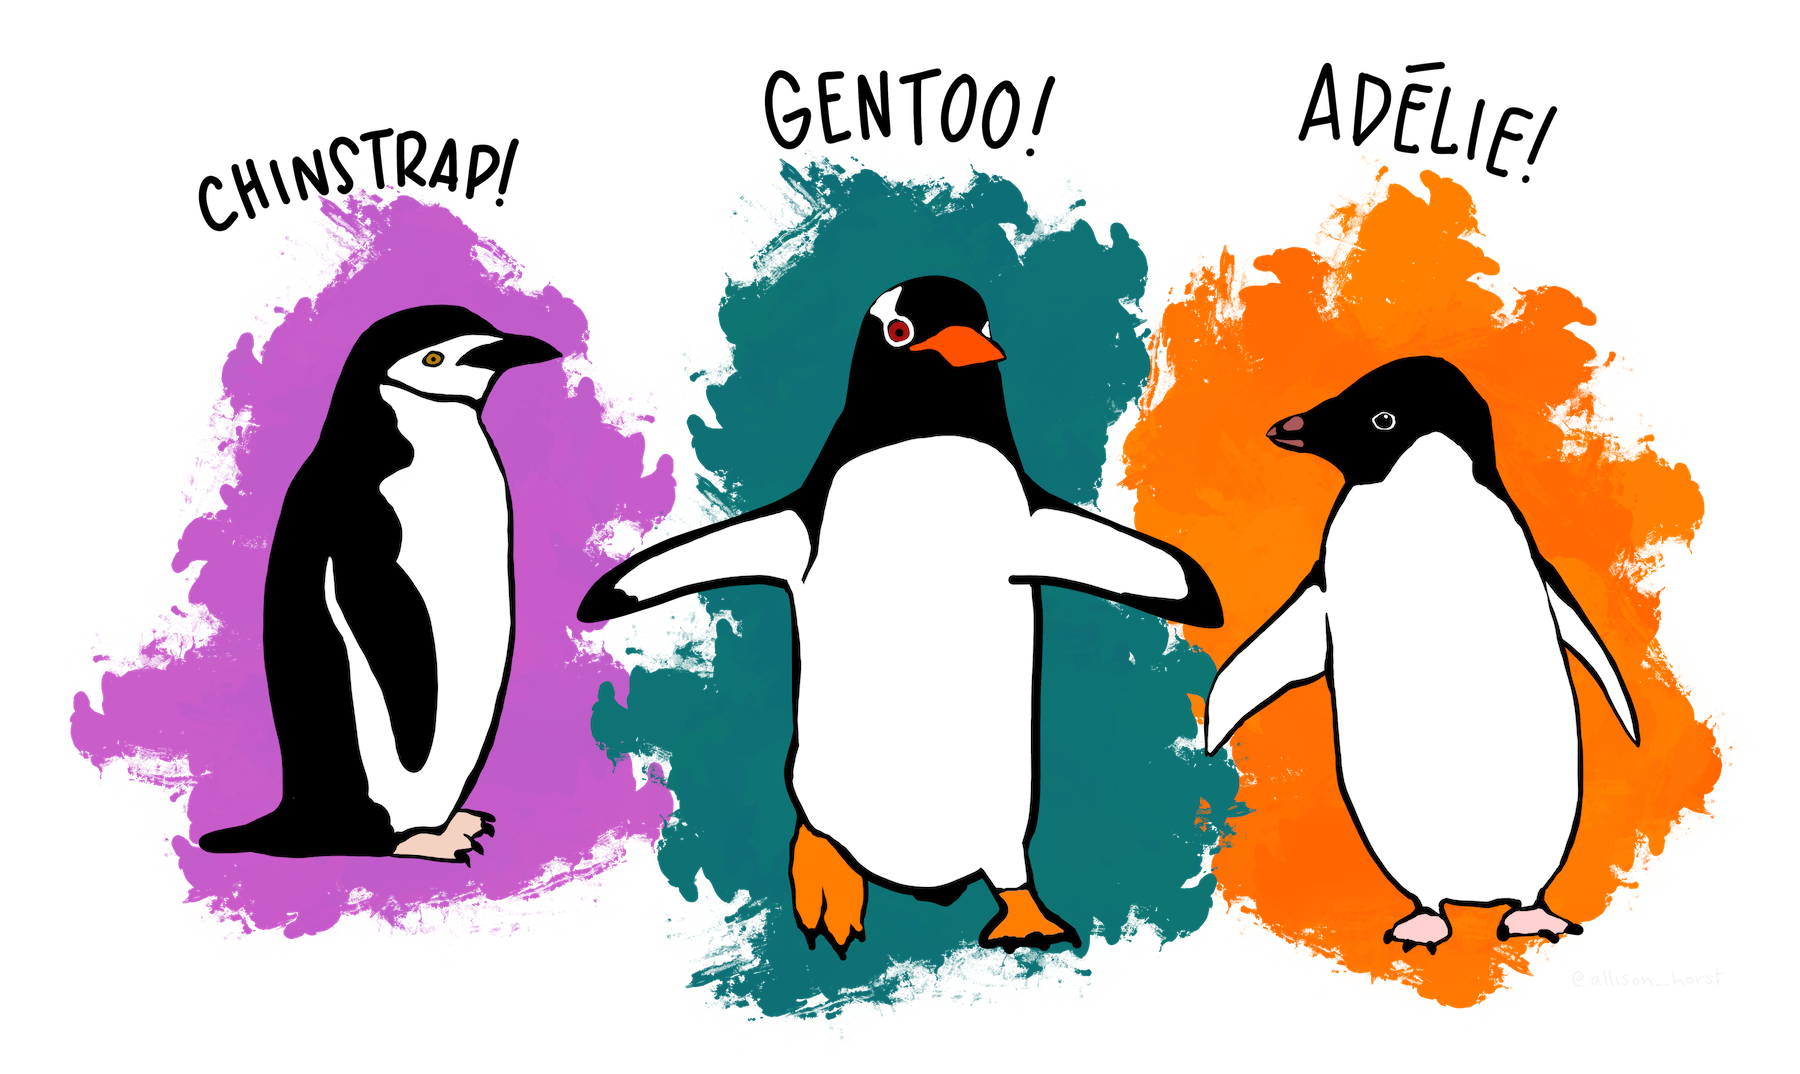
\includegraphics[height=0.36\textheight]{lter_penguins.png}\\[2pt]
    \creditoHorst
  }{%
    \begin{tikzpicture}[scale=0.8]
      \begin{scope}[shift={(-2.4,0)}] \pingAdelie \end{scope}
      \begin{scope}[shift={(0,0)}] \pingChinstrap \end{scope}
      \begin{scope}[shift={(2.4,0)}] \pingGentoo \end{scope}
    \end{tikzpicture}
  }

  \vspace{0.6cm}
  {\Large\color{azulUS} ¿Preguntas?}\\[10pt]

  \vspace{0.7cm}
  {\tiny\color{grisT}
  Datos: Horst A, Hill A, Gorman K (2020). \textit{palmerpenguins} (CC-0). ---
  Estudio original: Gorman KB, Williams TD, Fraser WR (2014).
  \textit{Ecological sexual dimorphism and environmental variability within a community
  of Antarctic penguins (genus Pygoscelis)}. PLoS ONE 9(3):e90081. ---
  Ilustraciones: \textit{Artwork by @allison\_horst}.}
\end{frame}
\end{document}